% Appendix Template
\section{Additional Temporal Tweezers} % Main appendix title
\label{AppendixC} % Change X to a consecutive letter; for referencing thI_{\sigma} appendix elsewhere, use \ref{AppendixX}

In this Appendix, we present additional tweezing results for the full LL Eq.~(\ref{eq:LLETweeze}) with the same analysis presented in Sec.~\ref{section:TweezeResults}. 

\subsection{Tweezer with Narrow  Width} 
\label{section:Skinny}


%%%%%%%%%% Fig  %%%%%%%%%%%%%%%%%%%%%%%%%%%%%%%%%%%%%%
\begin{figure}[htb!]
\centering 
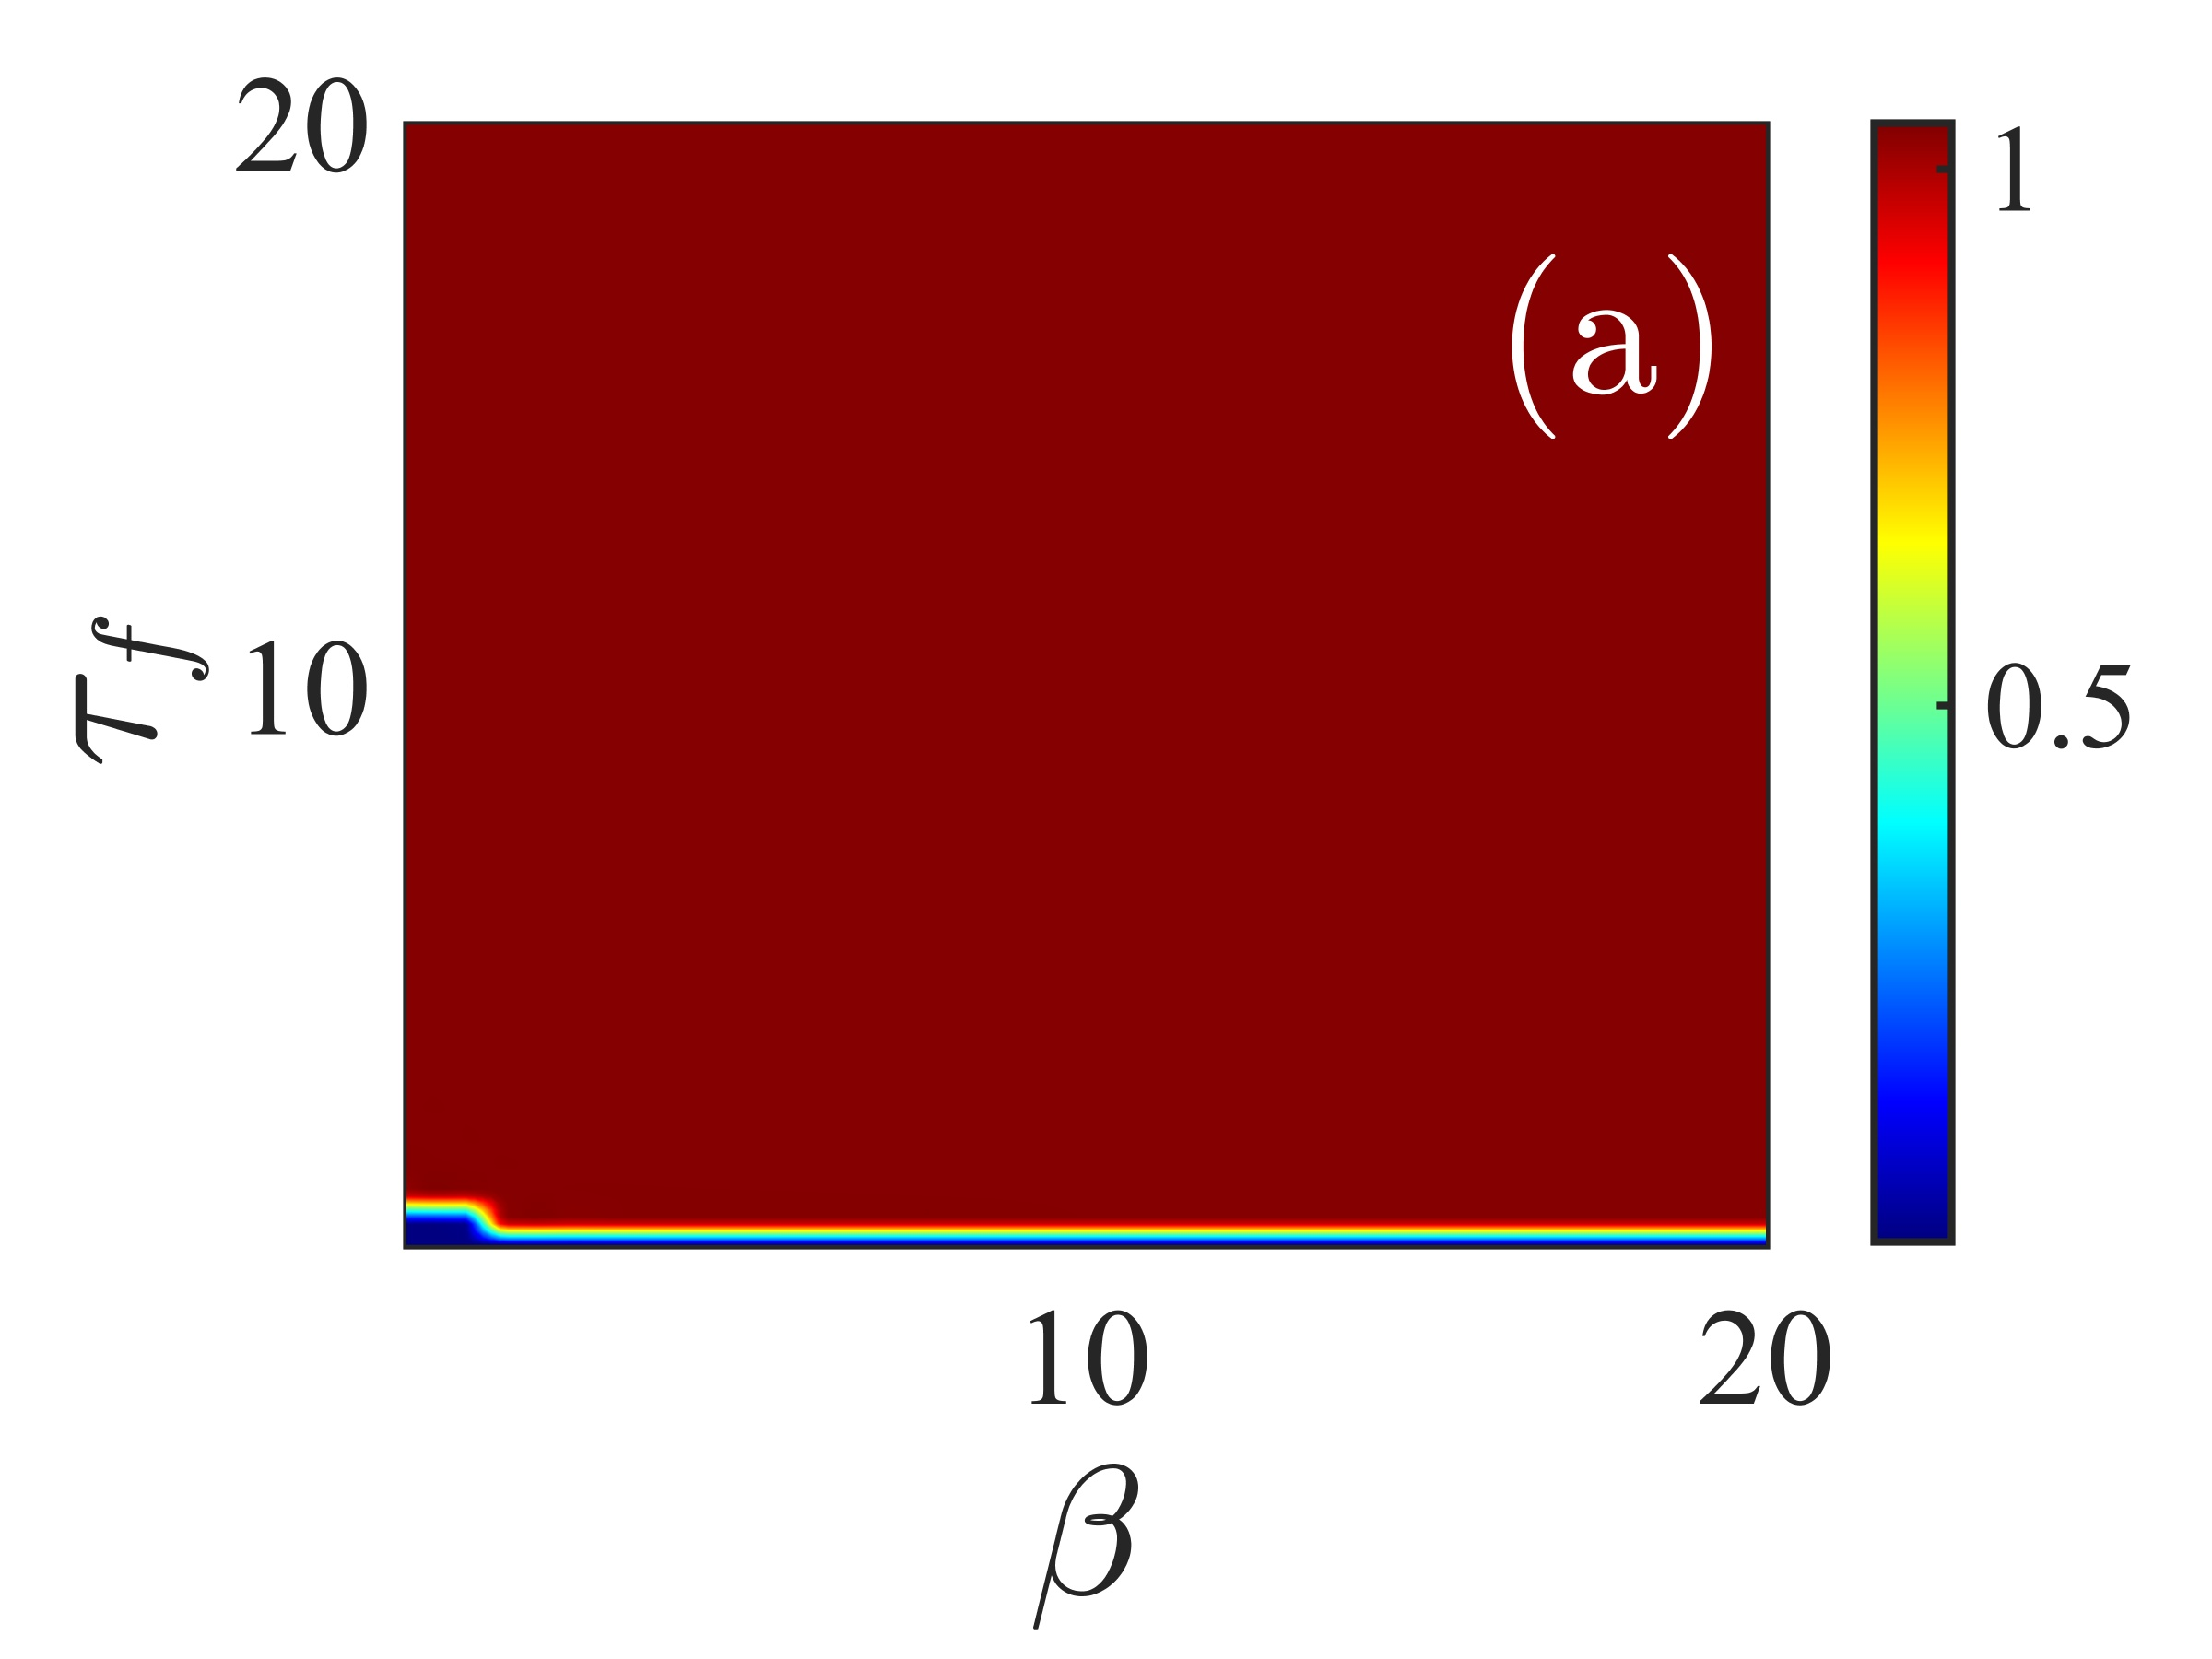
\includegraphics[width=4.2cm]{SkinnyQIn.jpg}
\hskip -0.5em 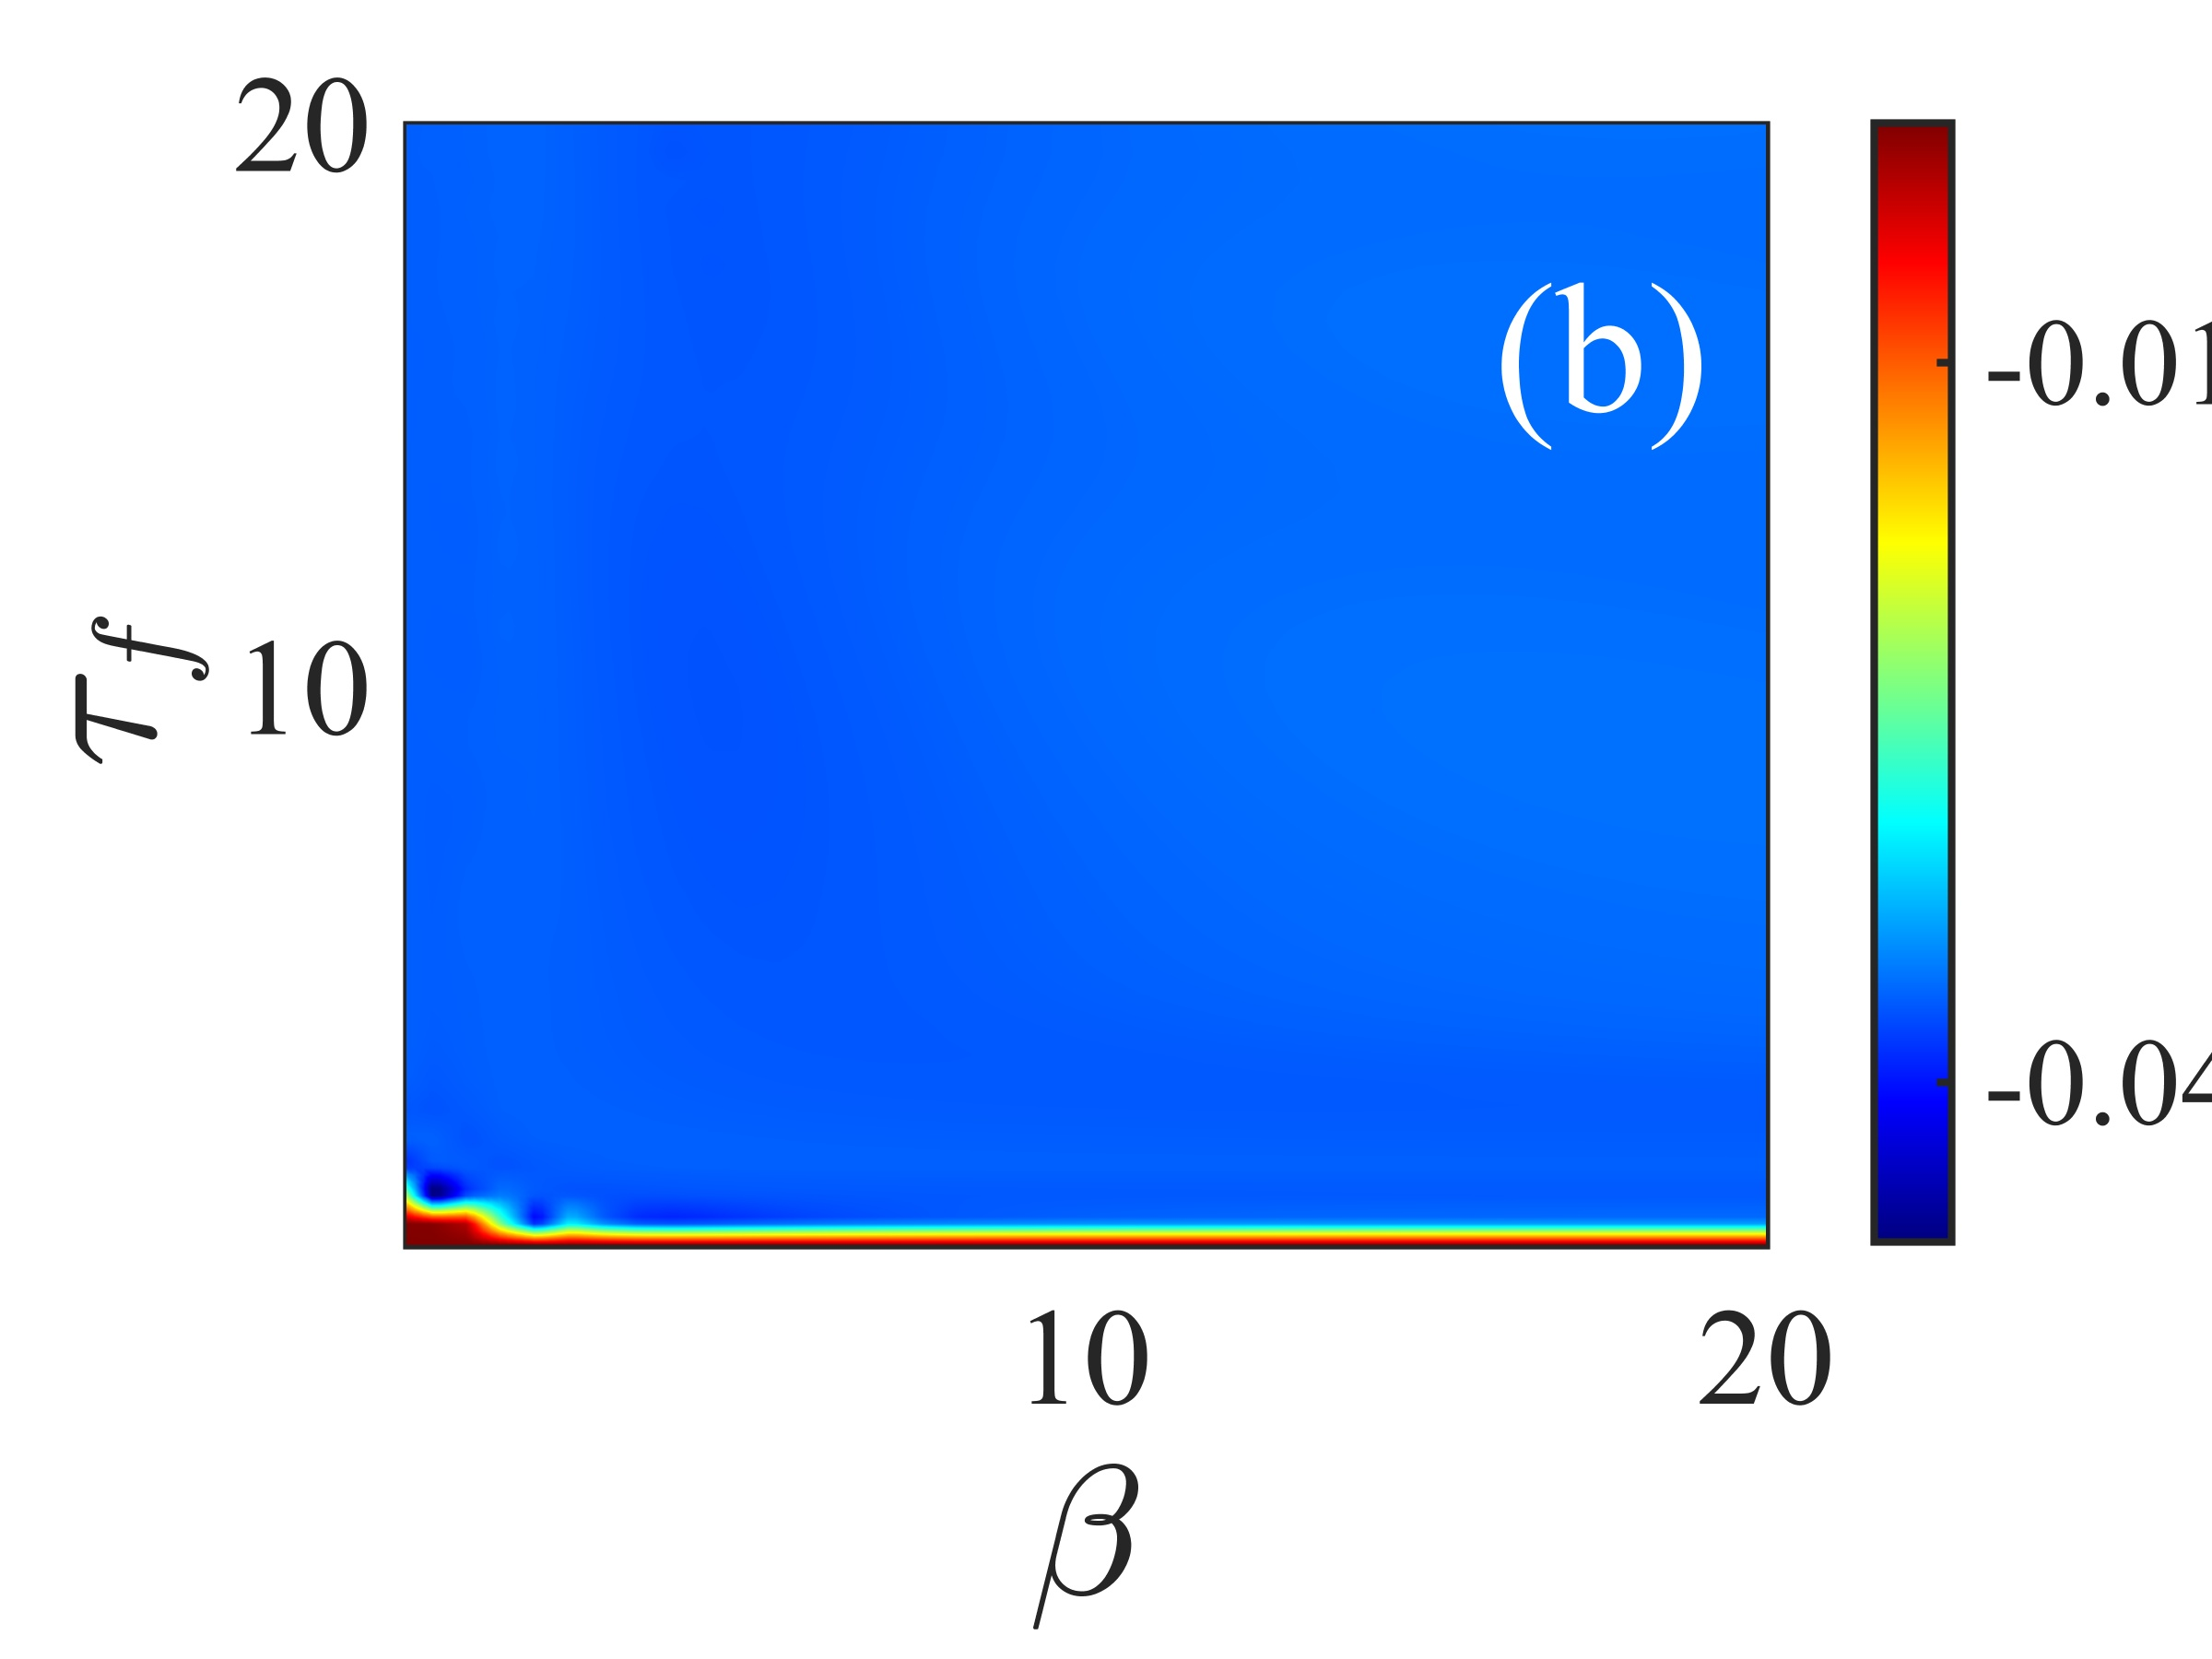
\includegraphics[width=4.2cm]{SkinnyQOut.jpg} \\
\hskip - 1em 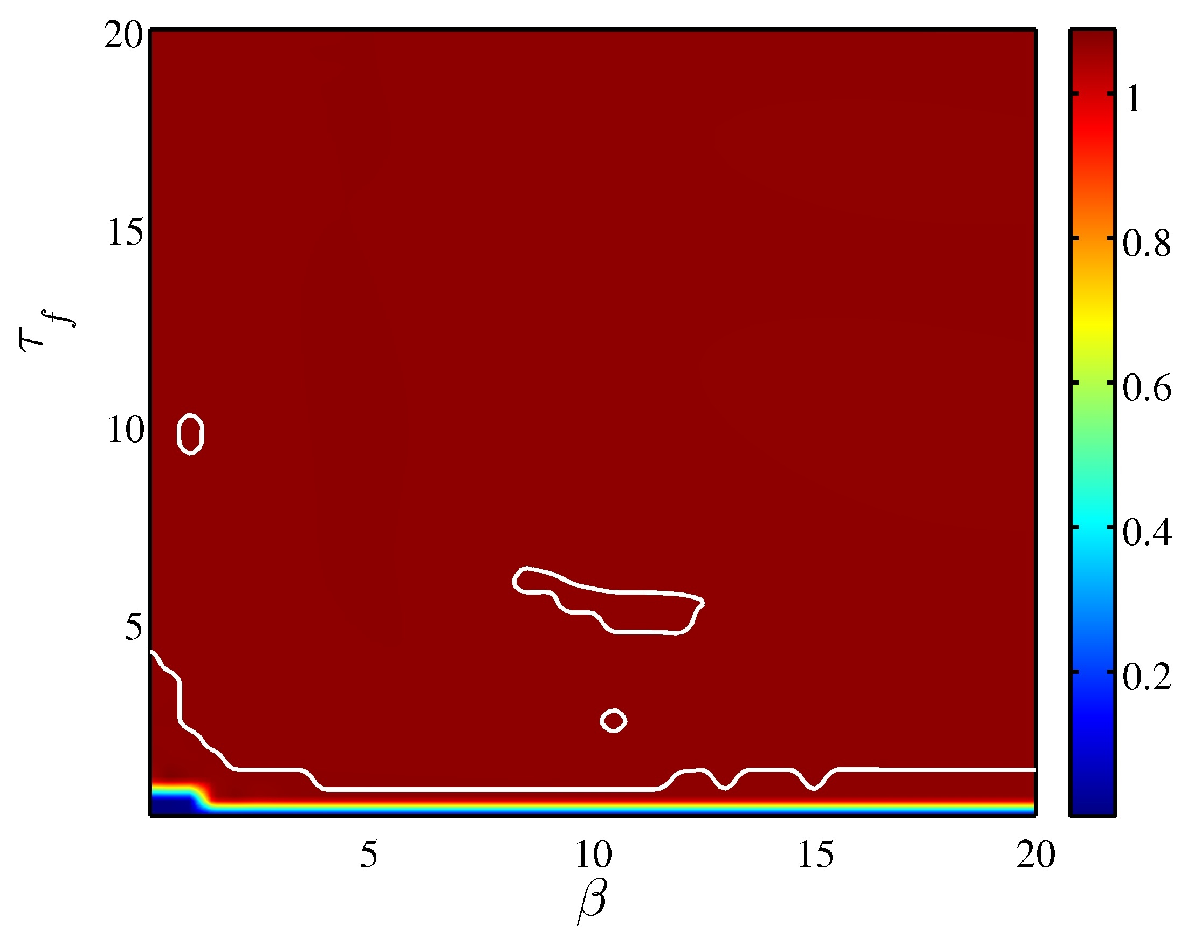
\includegraphics[width=8.5cm]{SkinnyPDEvODE_rcg_t.eps} 
\vspace{-0.5em}
\caption[Power Ratios Inside and Outside Tweezer with Narrow Width]{The density of the power ratios (a) inside and (b) outside of a narrow tweezer width $\sigma_\phi = 1$ and height $h_\phi = 2.3316$.  The detuning for the system is $\Delta =  4.1692$ and each combination of parameter is evolved for $z_f = 10 = 4z^*$, with $z^* = 2.5$.  (a) The power ratio density inside the tweezer $Q_{\rm I}$, where blue ($Q_{\rm I}=0$) is complete power inside the tweezer at $z_f$ and red ($Q_{\rm I}=1$) is no power inside the tweezer at $z_f$.  (b) The power ratio density outside the tweezer $Q_{\rm O}$, where $Q_{\rm O}$ = 0 depicts no change in power.   (c) 
The density of the difference of power ratios inside of a narrow tweezer, $Q_{\rm I} - Q_{\rm O}$ for the full LL model with a single contour at 0.5 (white line) for the NCVA threshold between tweezed and non-tweezed states.  For the difference of power ratios, a value of 1 is a non-tweezed CS, a value of 0.5 is a no-CS, and a value of 0 is a tweezed-CS.  The white contour line distinguishes the NCVA region between a solutions with tweezed CS and dissipative solutions with no-CS.  For the narrow width tweezer, the full LL model has a very small region of tweezed-CS for $\tau_f \le 0.1$, while the NCVA tweezed-CS region is $\tau_f \le 0.5$ with other islands of tweezability. 
}
\label{fig:SkinnyQ}
\end{figure}
%%%%%%%%%% Fig  %%%%%%%%%%%%%%%%%%%%%%%%%%%%%%%%%%%%%%


%%%%%%%%%% Fig  %%%%%%%%%%%%%%%%%%%%%%%%%%%%%%%%%%%%%%
\begin{figure}[htb!]
\centering
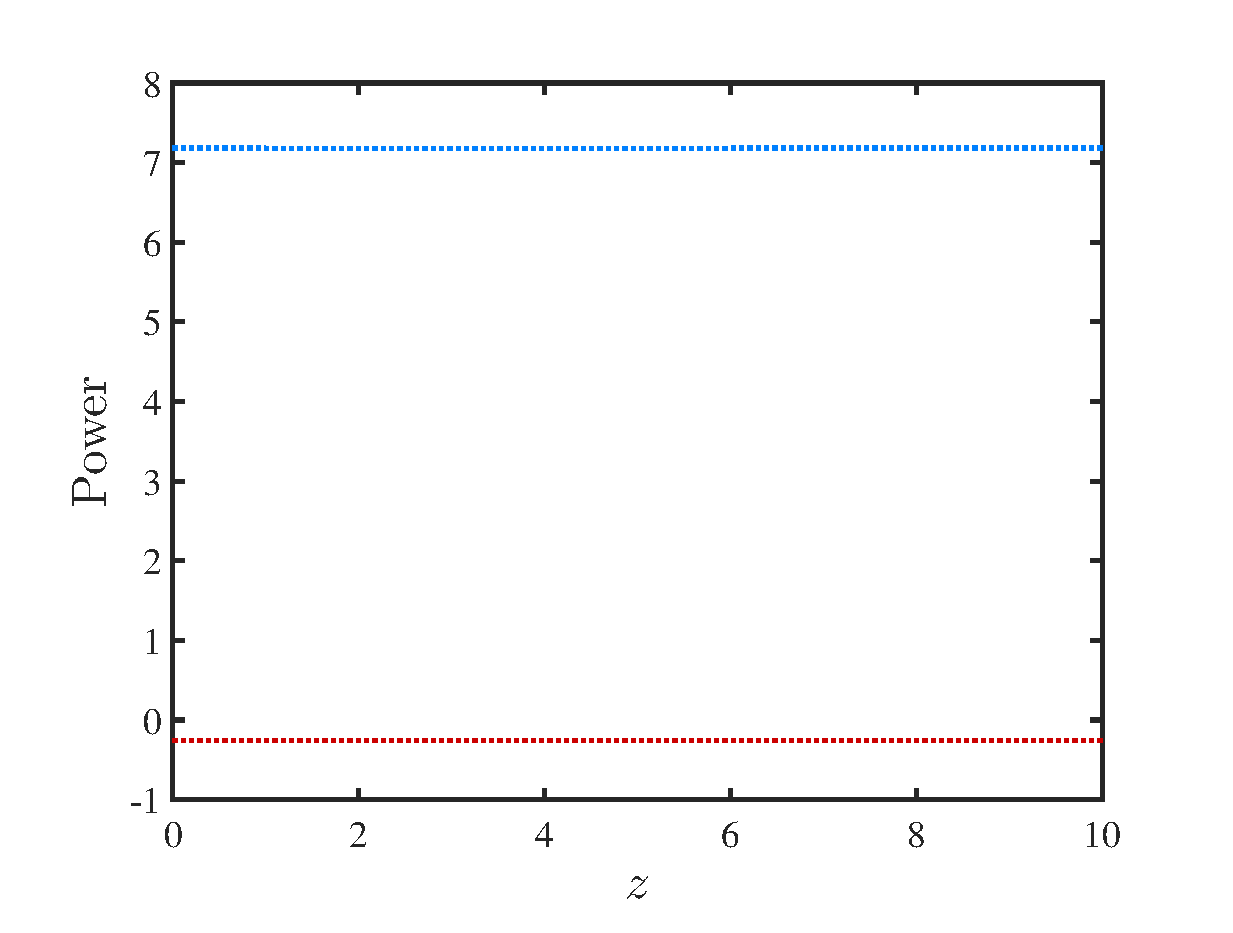
\includegraphics[width=4.2cm]{skinnyTimeMass1.eps} 
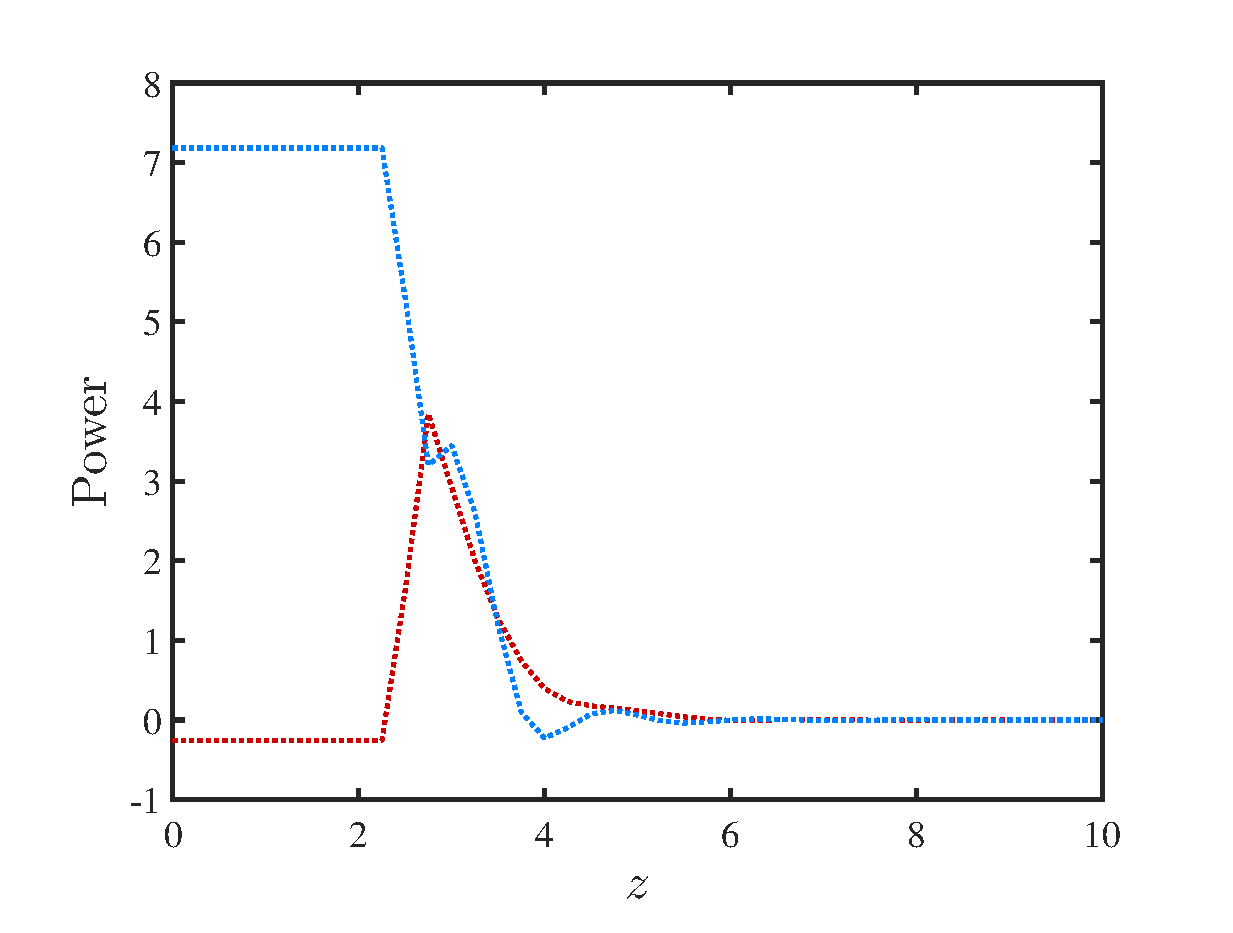
\includegraphics[width=4.2cm]{skinnyTimeMass3.eps} 
\caption[Tweezer with Narrow Width Power Comparison]{Comparison of the powers found inside the tweezer $P_{\rm I}$ (red line) and outside the tweezer $P_{\rm O}$ (blue line) for the parameters (a) $\tau_f = 0.1$ and $\beta=0.1$, with no change in power inside or outside the tweezer which describes a tweezed CS and (b) $\tau_f = 2$ and $\beta = 10$, with no change in power outside the tweezer and complete loss of power inside the tweezer describes a dissipative no-CS solution.  
}
\label{fig:SkinnyComp}
\end{figure}
%%%%%%%%%% Fig  %%%%%%%%%%%%%%%%%%%%%%%%%%%%%%%%%%%%%%

%%%%%%%%%% Fig  %%%%%%%%%%%%%%%%%%%%%%%%%%%%%%%%%%%%%%
%\begin{figure}[htb!]
%\centering
%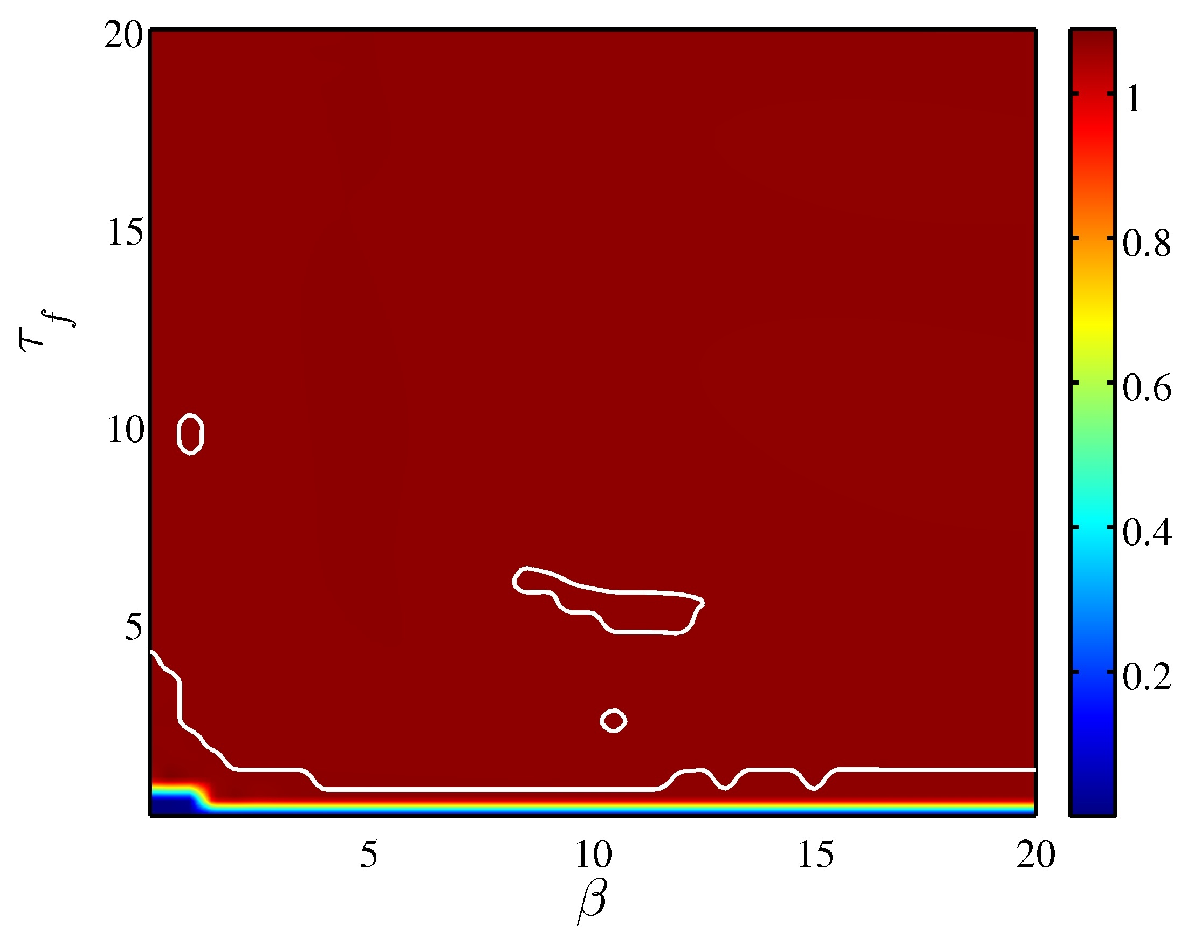
\includegraphics[width=8.5cm]{SkinnyPDEvODE_rcg_t.eps}
%\caption[Comparison of Power Ratio Inside Narrow Tweezer for LL Model and NCVA]{The density of the difference of power ratios inside of a narrow tweezer in the parameter space of $\tau_0$ for the full LL model (same as Fig.~{fig:SkinnyQ}(c)) with a single contour at 0.5 (white line) for the NCVA threshold between tweezed and non-tweezed states.  For the difference of power ratios, a value of 1 is a non-tweezed CS, a value of 0.5 is a no-CS, and a value of 0 is a tweezed-CS.  The white contour line distinguishes the NCVA region between a solutions with tweezed CS and dissipative solutions with no-CS.  For the narrow width tweezer, the full LL model has a very small region of tweezed-CS for $\tau_f \le 0.1$, while the NCVA tweezed-CS region is $\tau_f \le 0.5$ with other islands of tweezability. 
%}
%\label{fig:SkinnyVsNCVA}
%\end{figure}
%%%%%%%%%% Fig  %%%%%%%%%%%%%%%%%%%%%%%%%%%%%%%%%%%%%%

%%%%%%%%%% Fig  %%%%%%%%%%%%%%%%%%%%%%%%%%%%%%%%%%%%%%
\begin{figure}[b!]
\centering
\hskip 0.4em 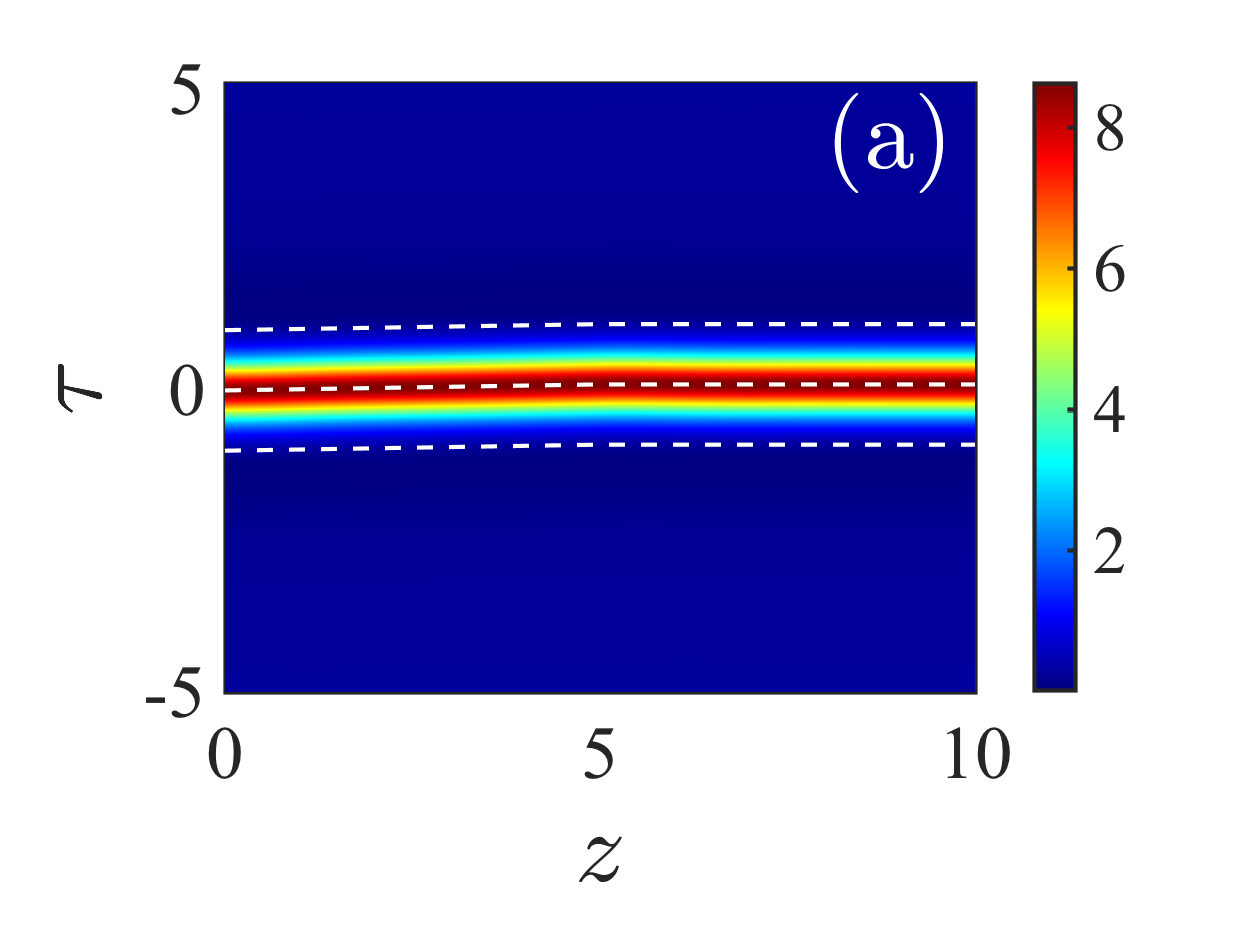
\includegraphics[width=4.2cm]{skinnyDensity1.eps} 
\hskip -0.5em 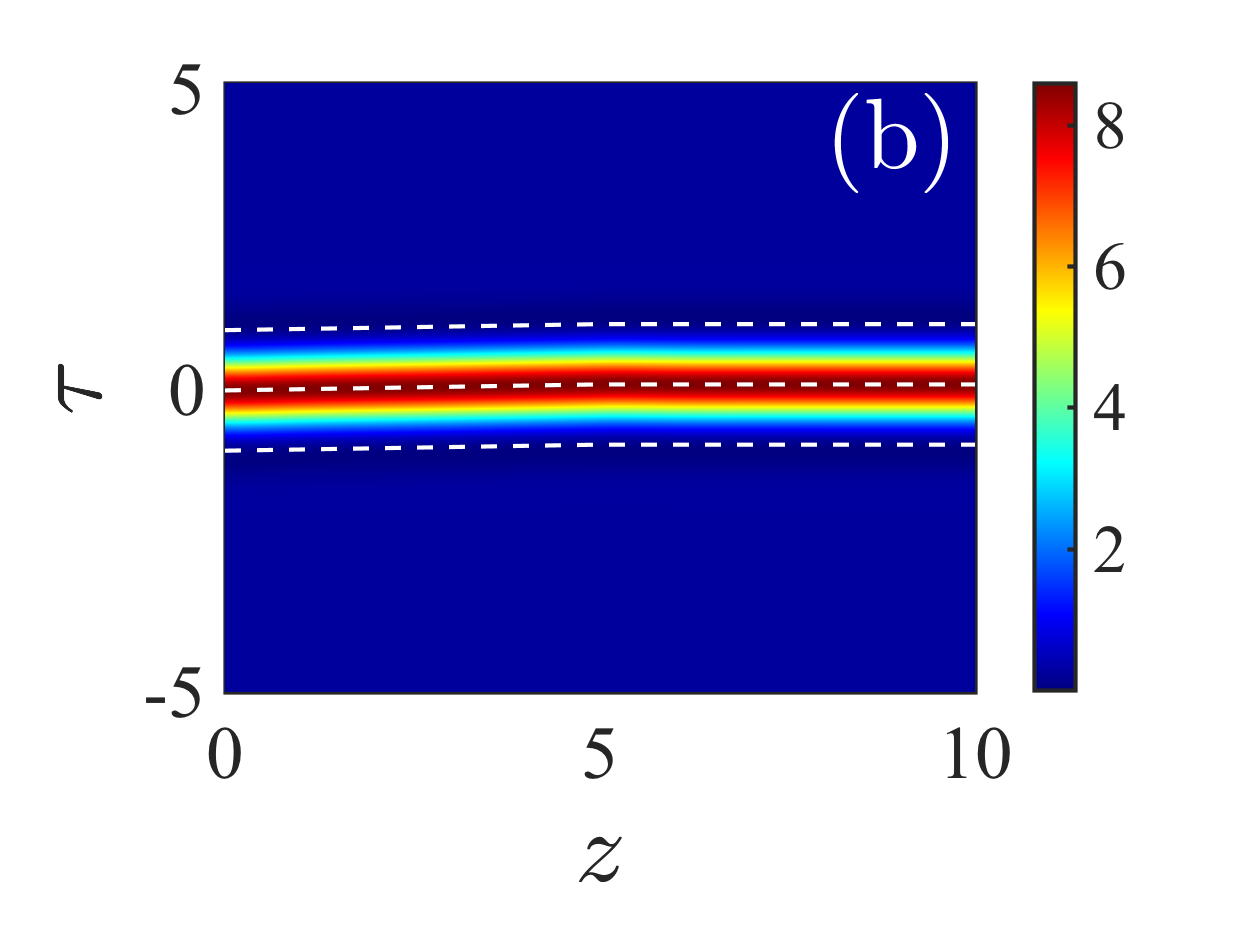
\includegraphics[width=4.2cm]{skinnyNCVADensity1.eps} 
\\
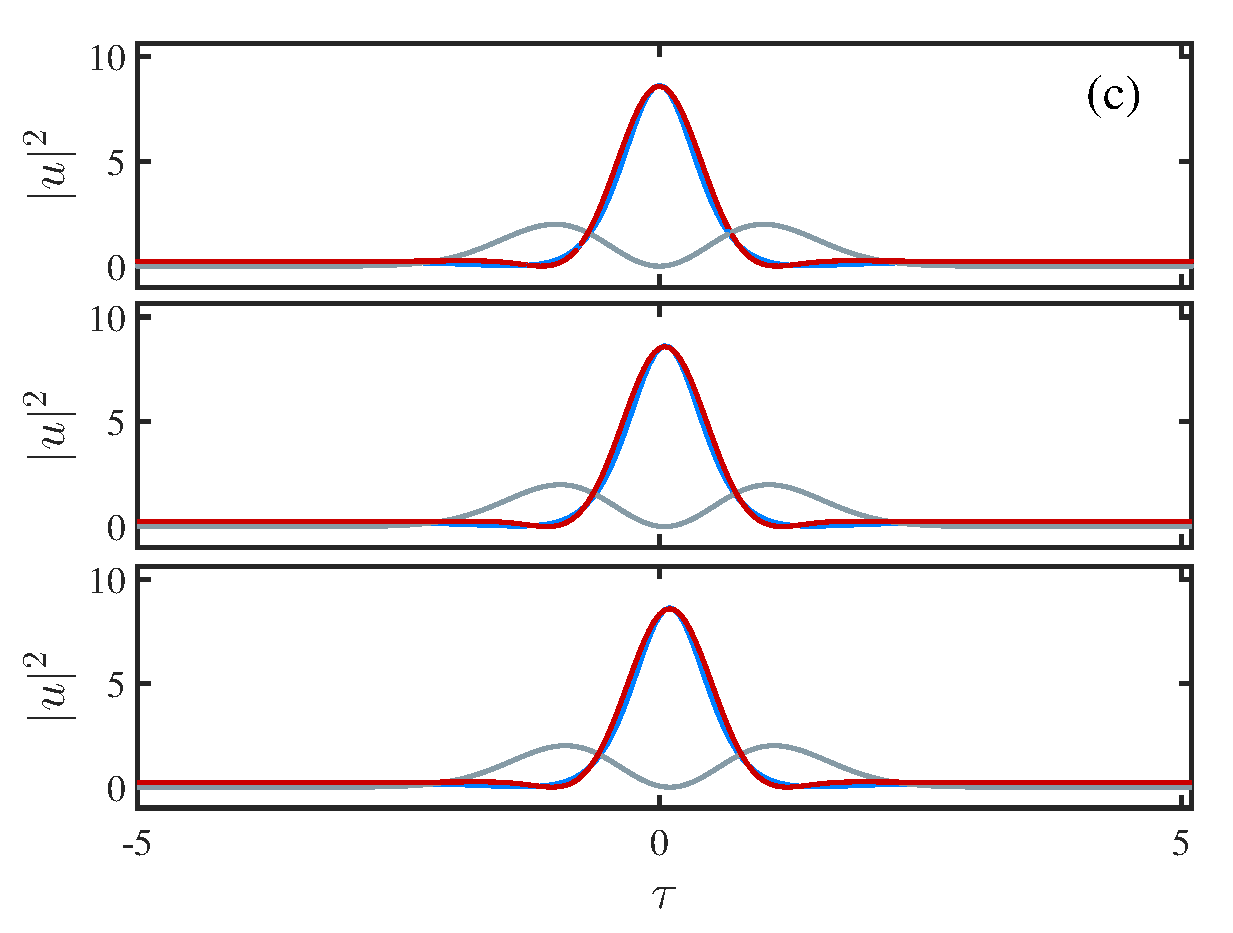
\includegraphics[width=8cm]{skinnyTimeSeries1.eps} 
\vspace{-0.5em}
\caption[Dynamic Evolution of Narrow Tweezer with Tweezed CS]{Example of the density evolution for the narrow tweezer state with $\tau_f = 0.1$ and $\beta = 0.1$ for the LL model (a) and NCVA (b) and (c) snapshots for the corresponding states of LL model (solid (blue) line), NCVA (solid (red) line) and effective potential depicted as solid (grey) line.  Evolution of steady state CS solution in narrow tweezer for $\tau_0(z)$ (dashed (white) line) for full LL model (a) and NCVA (b).  The initial steady state, see LL model solid (blue) and NCVA solid (red) in top panel (c) for $z = 0$ and the state while being tweezed at $z = z^* = 2.5$ depicted in solid (blue) LL model [solid (red) NCVA] in middle panel (c).  The bottom panel (c) is the state at $z = z_f = 10$.  Both the density evolution in the LL model and NCVA, as well as the snapshots, correspond to a tweezed CS that is manipulated by the narrow tweezer. 
}
\label{fig:Skinny1}
\end{figure}
%%%%%%%%%% Fig  %%%%%%%%%%%%%%%%%%%%%%%%%%%%%%%%%%%%%%

In the first case study, we are interested in a tweezer with a narrow width $\sigma_\phi = 1$ and height $h_\phi = 2.3316$ given by Eq.~(\ref{height}).  For the full LL Eq.~(\ref{eq:LLETweeze}), the steady state CS is found centered at $\tau_0 = 0$ using a Newton-Krylov solver and the power-balance constraint Eq.~(\ref{LLConstraint}) which selects a detuning parameter value of $\Delta =  4.1692$.  The same $\Delta$, $\sigma_\phi$, and $h_\phi$ are used in the NCVA with a Newton-Krylov solver to find the initial variational parameters for the system.  The parameter space for $\beta$ and $\tau_f$ are discretized into 41 steps between 0.1 and 20, giving 1681 combinations for $\tau_0(z)$ [Eq.~(\ref{tau0})].  The full LL Eq.~(\ref{eq:LLETweeze}) is solved using a Runge-Kutta method in time and finite differences in space and the NCVA system of ODEs are solved using Matlab's ode15s.  It is important to note, the NCVA requires a stiff ODE solver to produce the numeric results. 
%Also, at this time we should mention the time-varying ode15s has a speedup of XX compared to fixed time ode15s.  There is also a XX speedup between the PDE Runge-Kutta solver and the ODE solver ode15s.  
Both the full LL equation and NCVA evolve until $z_f = 10 = 4z^*$, with $z^* = 2.5$ which ensures that the tweezed and/or non-tweezed CS have enough time to converge towards their steady state. 


%%%%%%%%%% Fig  %%%%%%%%%%%%%%%%%%%%%%%%%%%%%%%%%%%%%%
\begin{figure}[t!]
\centering
\hskip 0.4em 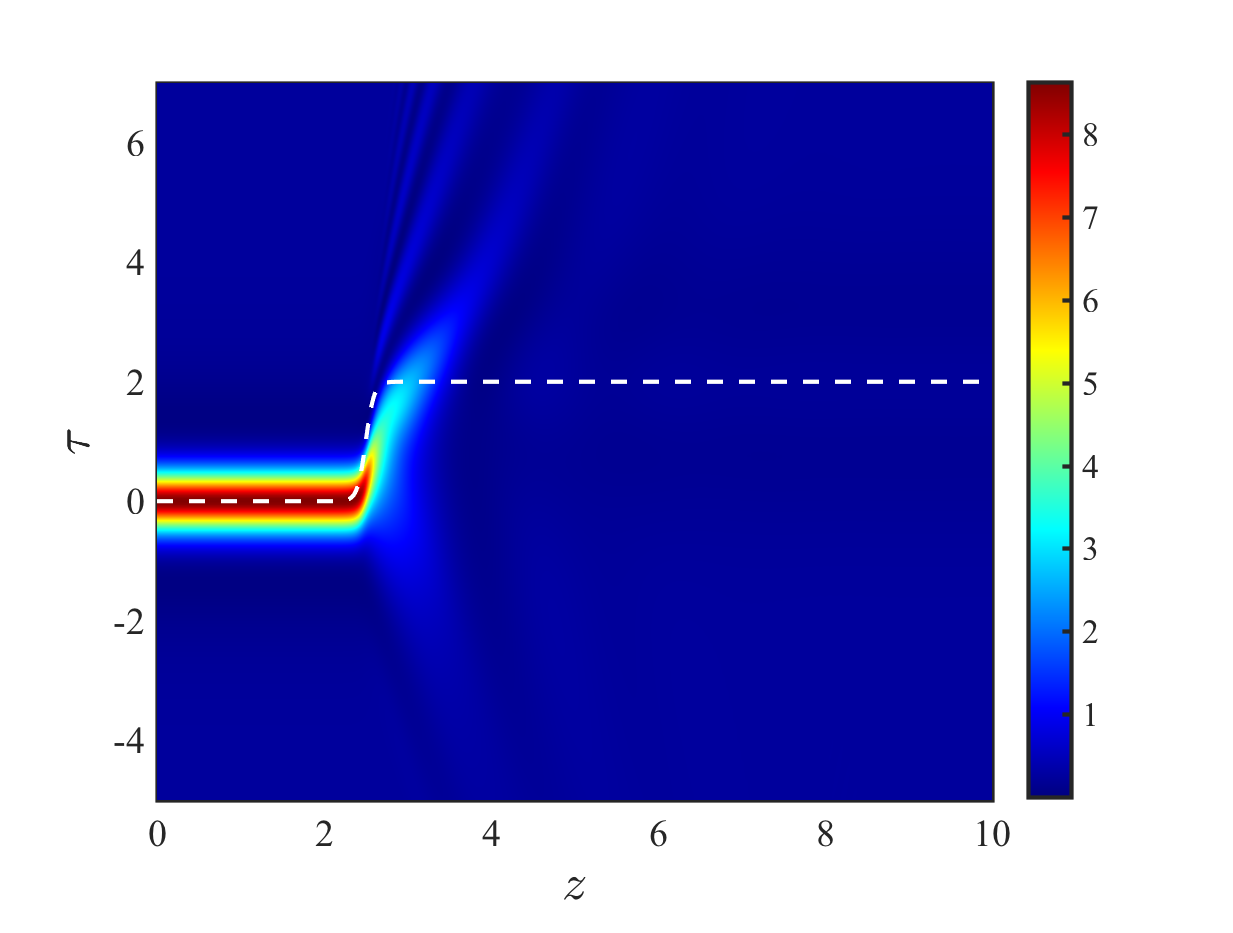
\includegraphics[width=4.2cm]{skinnyDensity3.eps} 
\hskip -0.5em 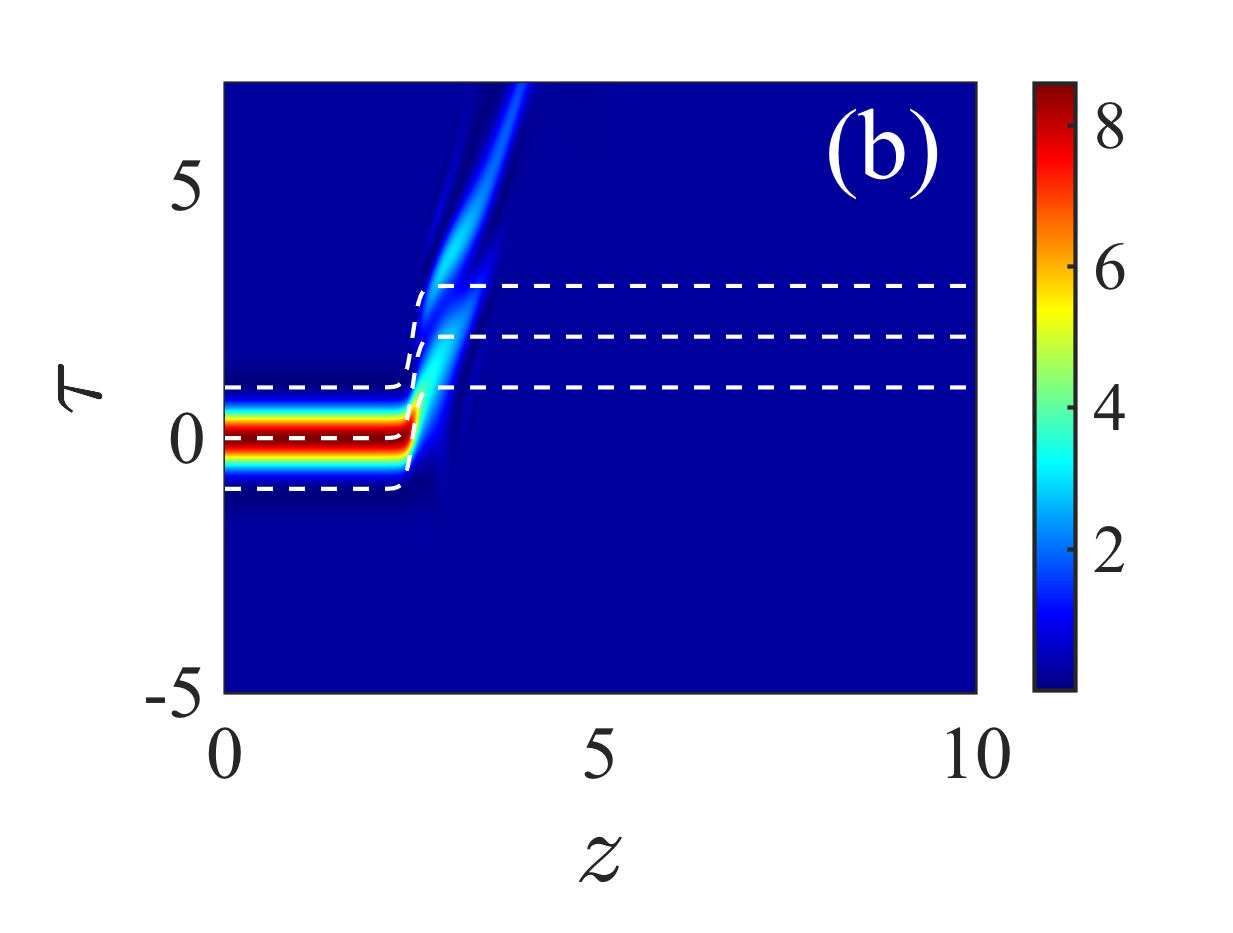
\includegraphics[width=4.2cm]{skinnyNCVADensity3.eps} 
\\
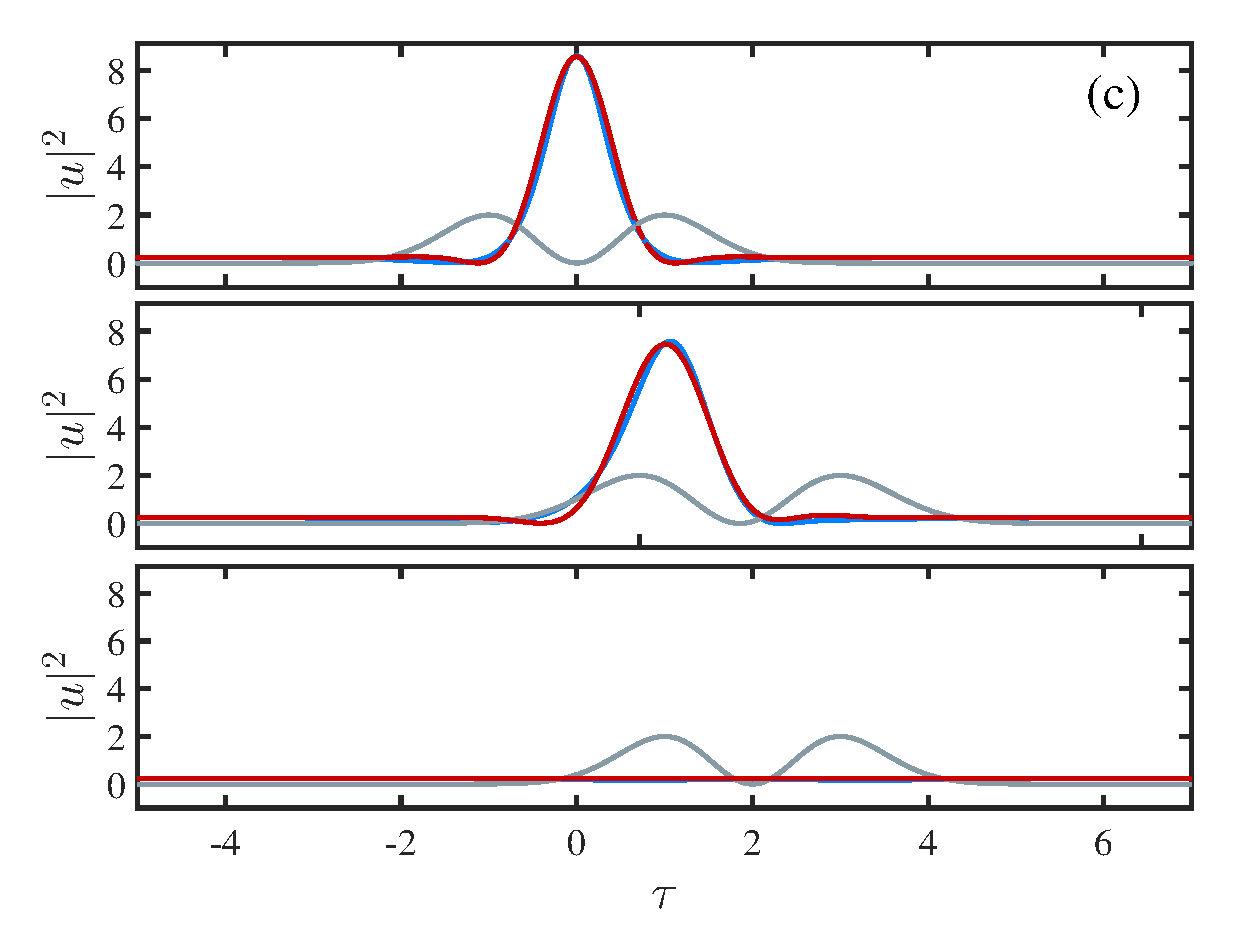
\includegraphics[width=8cm]{skinnyTimeSeries3.eps} 
\vspace{-0.5em}
\caption[Dynamic Evolution of Narrow Tweezer with no-CS]{Dynamic evolution as in Fig.~\ref{fig:Skinny1} but for $\tau_f = 2$ and $\beta = 10$.  Same layout as in Fig.~\ref{fig:Skinny1}.  In this sample, both the LL model solution and NCVA are a no-CS.
}
\label{fig:Skinny2}
\end{figure}
%%%%%%%%%% Fig  %%%%%%%%%%%%%%%%%%%%%%%%%%%%%%%%%%%%%%

As described above, we calculate $Q_{\rm I}$ from Eq.~(\ref{QIn}) and $Q_{\rm O}$ from Eq.~(\ref{QOut}) for all parameter combinations.  Figure~\ref{fig:SkinnyQ} depicts the density of these power ratios inside (Fig.~\ref{fig:SkinnyQ}(a)) and outside (Fig.~\ref{fig:SkinnyQ}(a)) the narrow tweezer.  In order to identify the different dynamical regions, both $Q_{\rm I}$ and $Q_{\rm O}$ need to be analyzed simultaneously.  For example $Q_{\rm I}$ = 0 is either a no-CS for $Q_{\rm O}=0$ or a non-tweezed CS for $Q_{\rm O}=1$.  For easier interpretation of the results, we use the difference in power ratios, $Q_{\rm diff} = Q_{\rm I} - Q_{\rm O}$, such that the values $Q_{\rm diff} = 0, 0.5$, and 1, respectively, represent tweezed-CS, no-CS, and non-tweezed CS.  Based on Fig.~\ref{fig:SkinnyQ}, the narrow tweezer is only defined by two fundamental states: a tweezed CS for all $\beta$ when $\tau_f \le 0.1$ and no-CS for all other parameters.  The threshold is very low for the existence of the tweezed CS, which is detrimental for the manipulation desired in a good tweezer.  The NCVA solutions only have two fundamental states: (i) a tweezed CS or (ii) a no-CS solution (there is no NCVA solution in which the tweezer leaves behind a CS).  Therefore, it is not necessary to use $Q_{\rm O}$ since both states result in $Q_{\rm O} \approx 0$.  Figure~\ref{fig:SkinnyQ} depicts a single contour (white line) of the $Q_{\rm diff} = 0.5$ superimposed on the same density of the full LL model.  This figure allows for a direct comparison of the threshold between a tweezed CS and no-CS solution of the NCVA (white line) and the state regions of the full LL model.  For the narrow tweezer, the NCVA solutions have a wider region for the existence tweezed CS than the LL model.  The NCVA also has islands of tweezed CS for larger values of $\tau_f$ and $\beta$ which do not exist in the full LL model.

In order to better explain the power ratio, we examine the power inside $P_{\rm I}$ Eq.~(\ref{Pin}) and outside $P_{\rm O}$ Eq.~(\ref{Pout}) for $\tau_f = 0.1$ with $\beta = 0.1$ and $\tau_f = 0.5$ with  $\beta=10$ in Fig.~\ref{fig:SkinnyComp}.  According to Fig.~\ref{fig:SkinnyQ}, for the example with $\beta = 0.5$ we have a tweezed CS and for $\beta = 10$ we have a no-CS.  By analyzing the power as a function of $z$ we can also determine the state of the system.  In Fig.~\ref{fig:SkinnyComp} the red lines depict $P_{\rm I}$ while the blue lines depict $P_{\rm O}$ for $\tau_f = 0.1$ with $\beta = 0.1$ (Fig.~\ref{fig:SkinnyComp}(a)) and $\tau_f = 0.5$ with $\beta=10$ (Fig.~\ref{fig:SkinnyComp}(b)).  For the former case, since there is no change in power inside or outside the narrow tweezer the CS is effectively tweezed.  In contrast, for the latter case, the complete loss of power inside the tweezer with no change in power outside the tweezer describes a dissipative no-CS solution.

%%%%%%%%%% Fig  %%%%%%%%%%%%%%%%%%%%%%%%%%%%%%%%%%%%%%
\begin{figure}[t!]
\centering
\hskip 0.4em 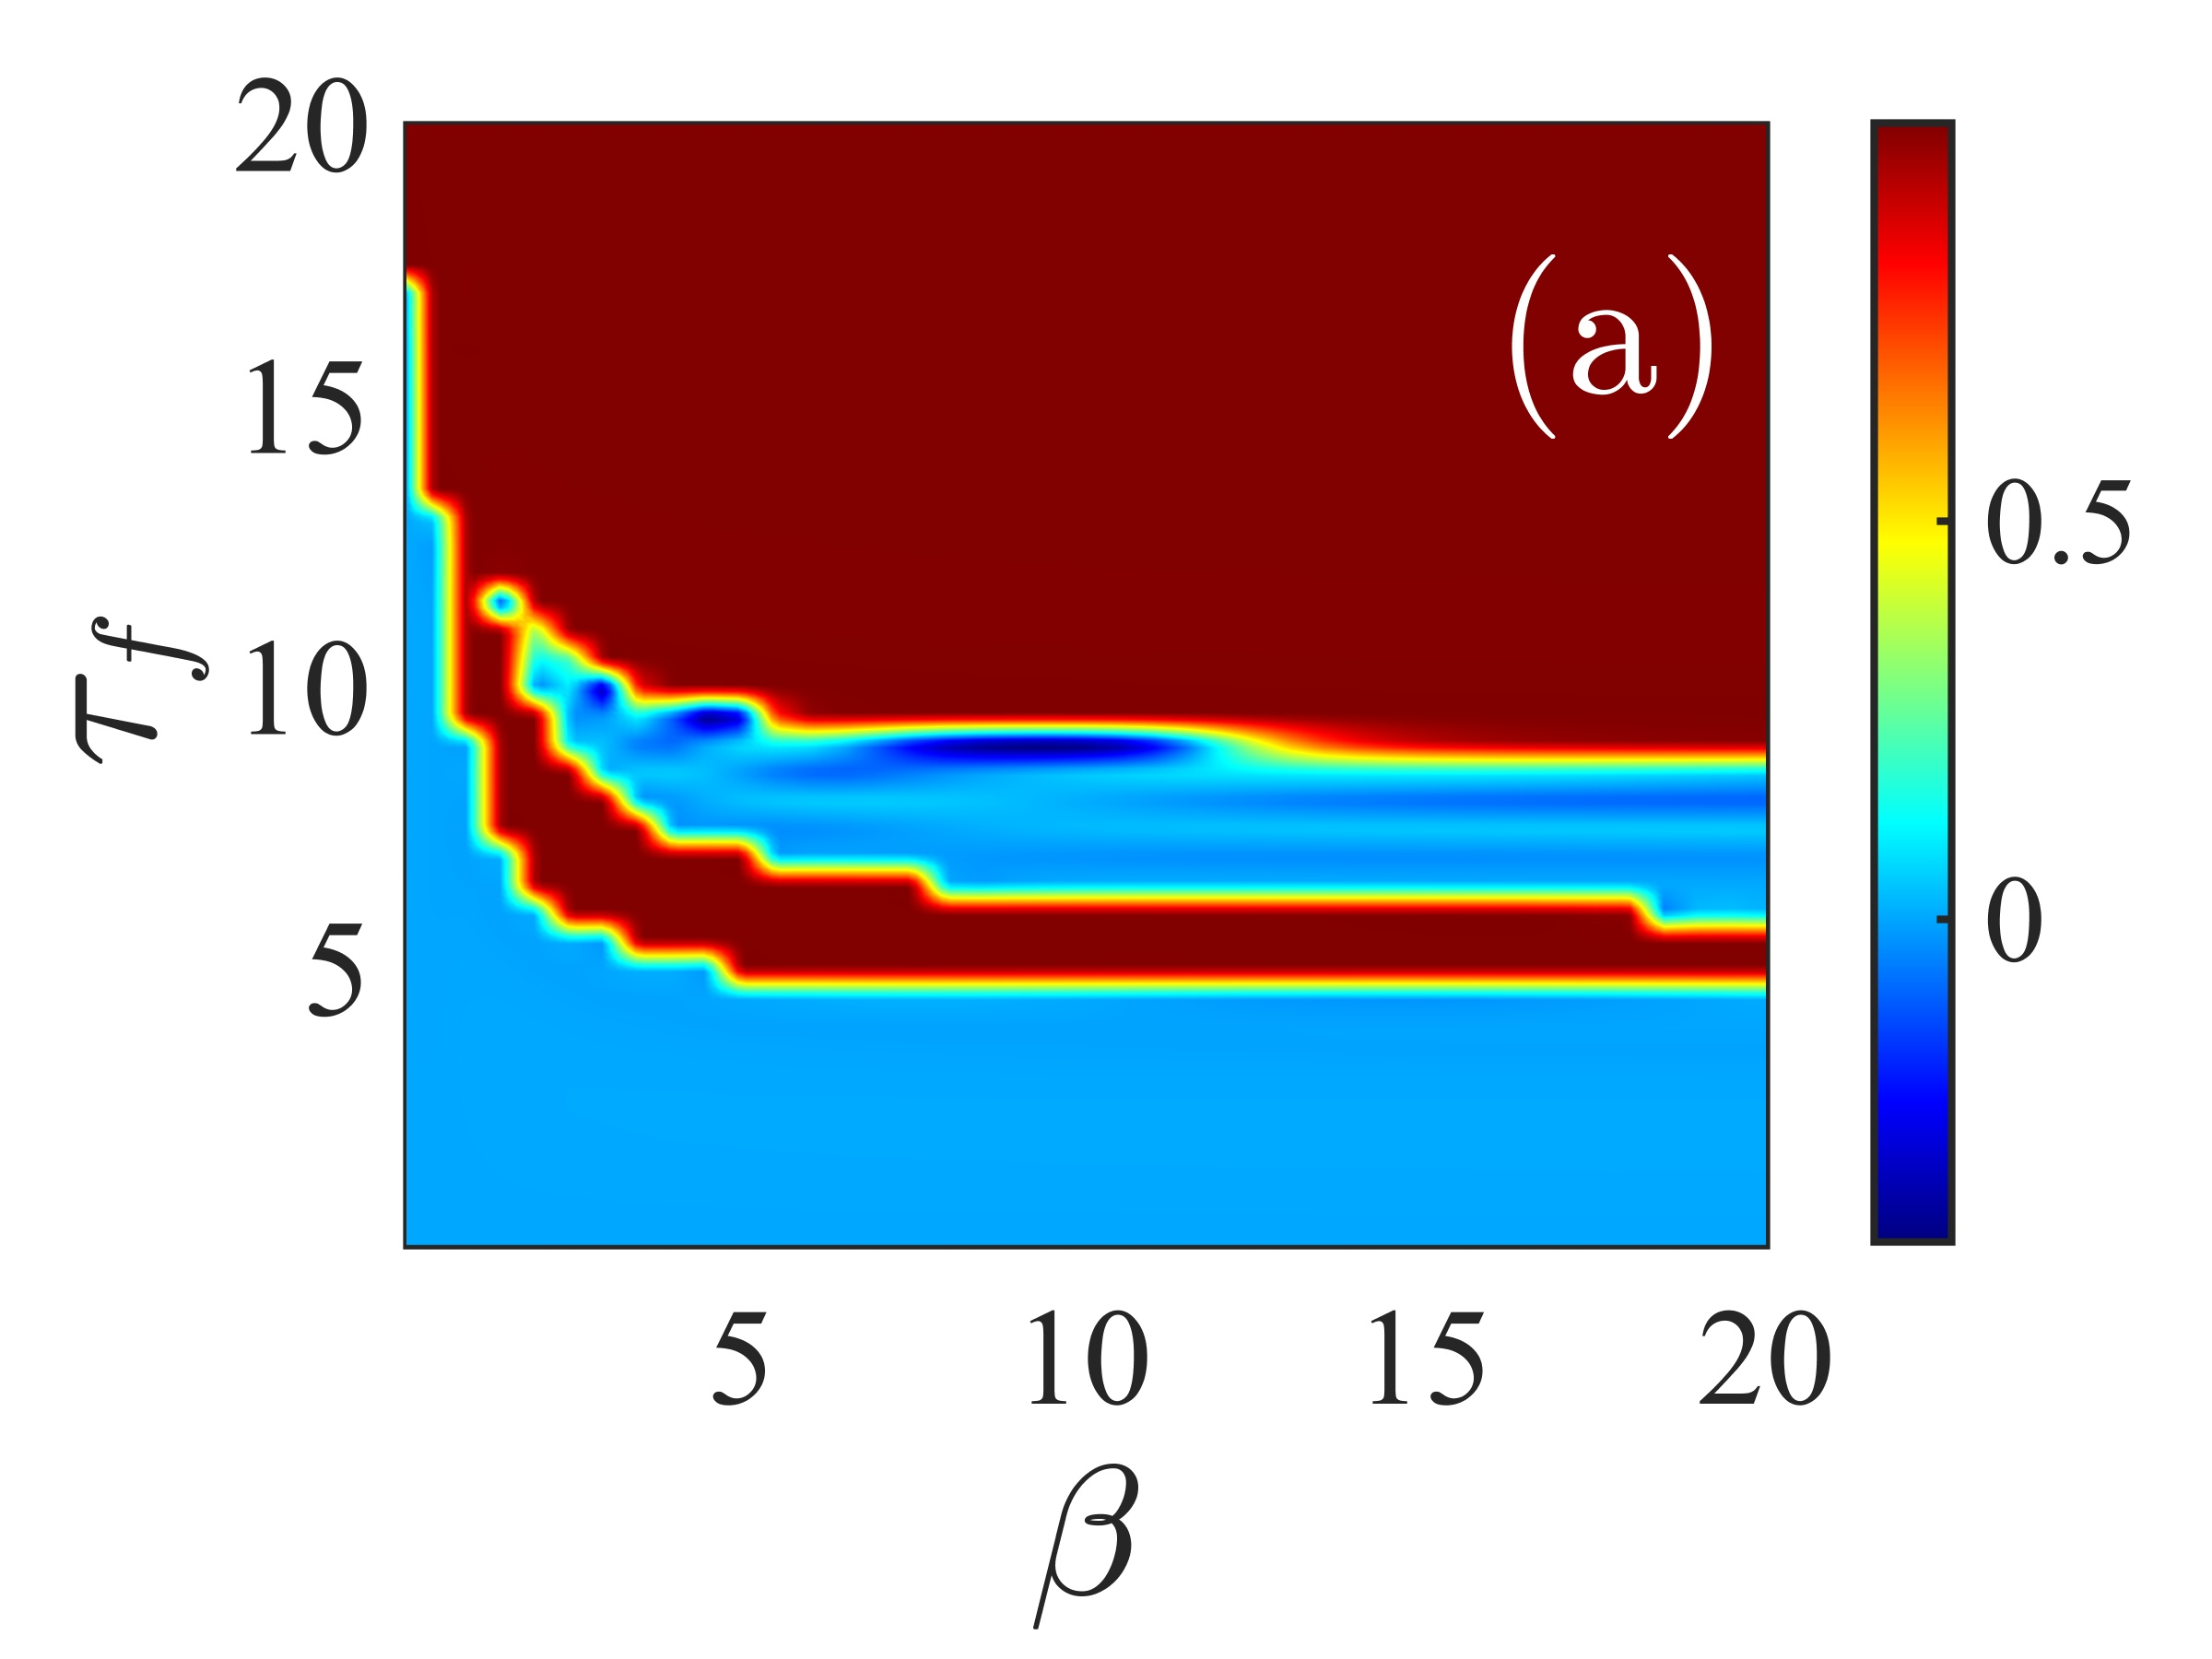
\includegraphics[width=4.2cm]{FatQIn.jpg}
\hskip -0.5em 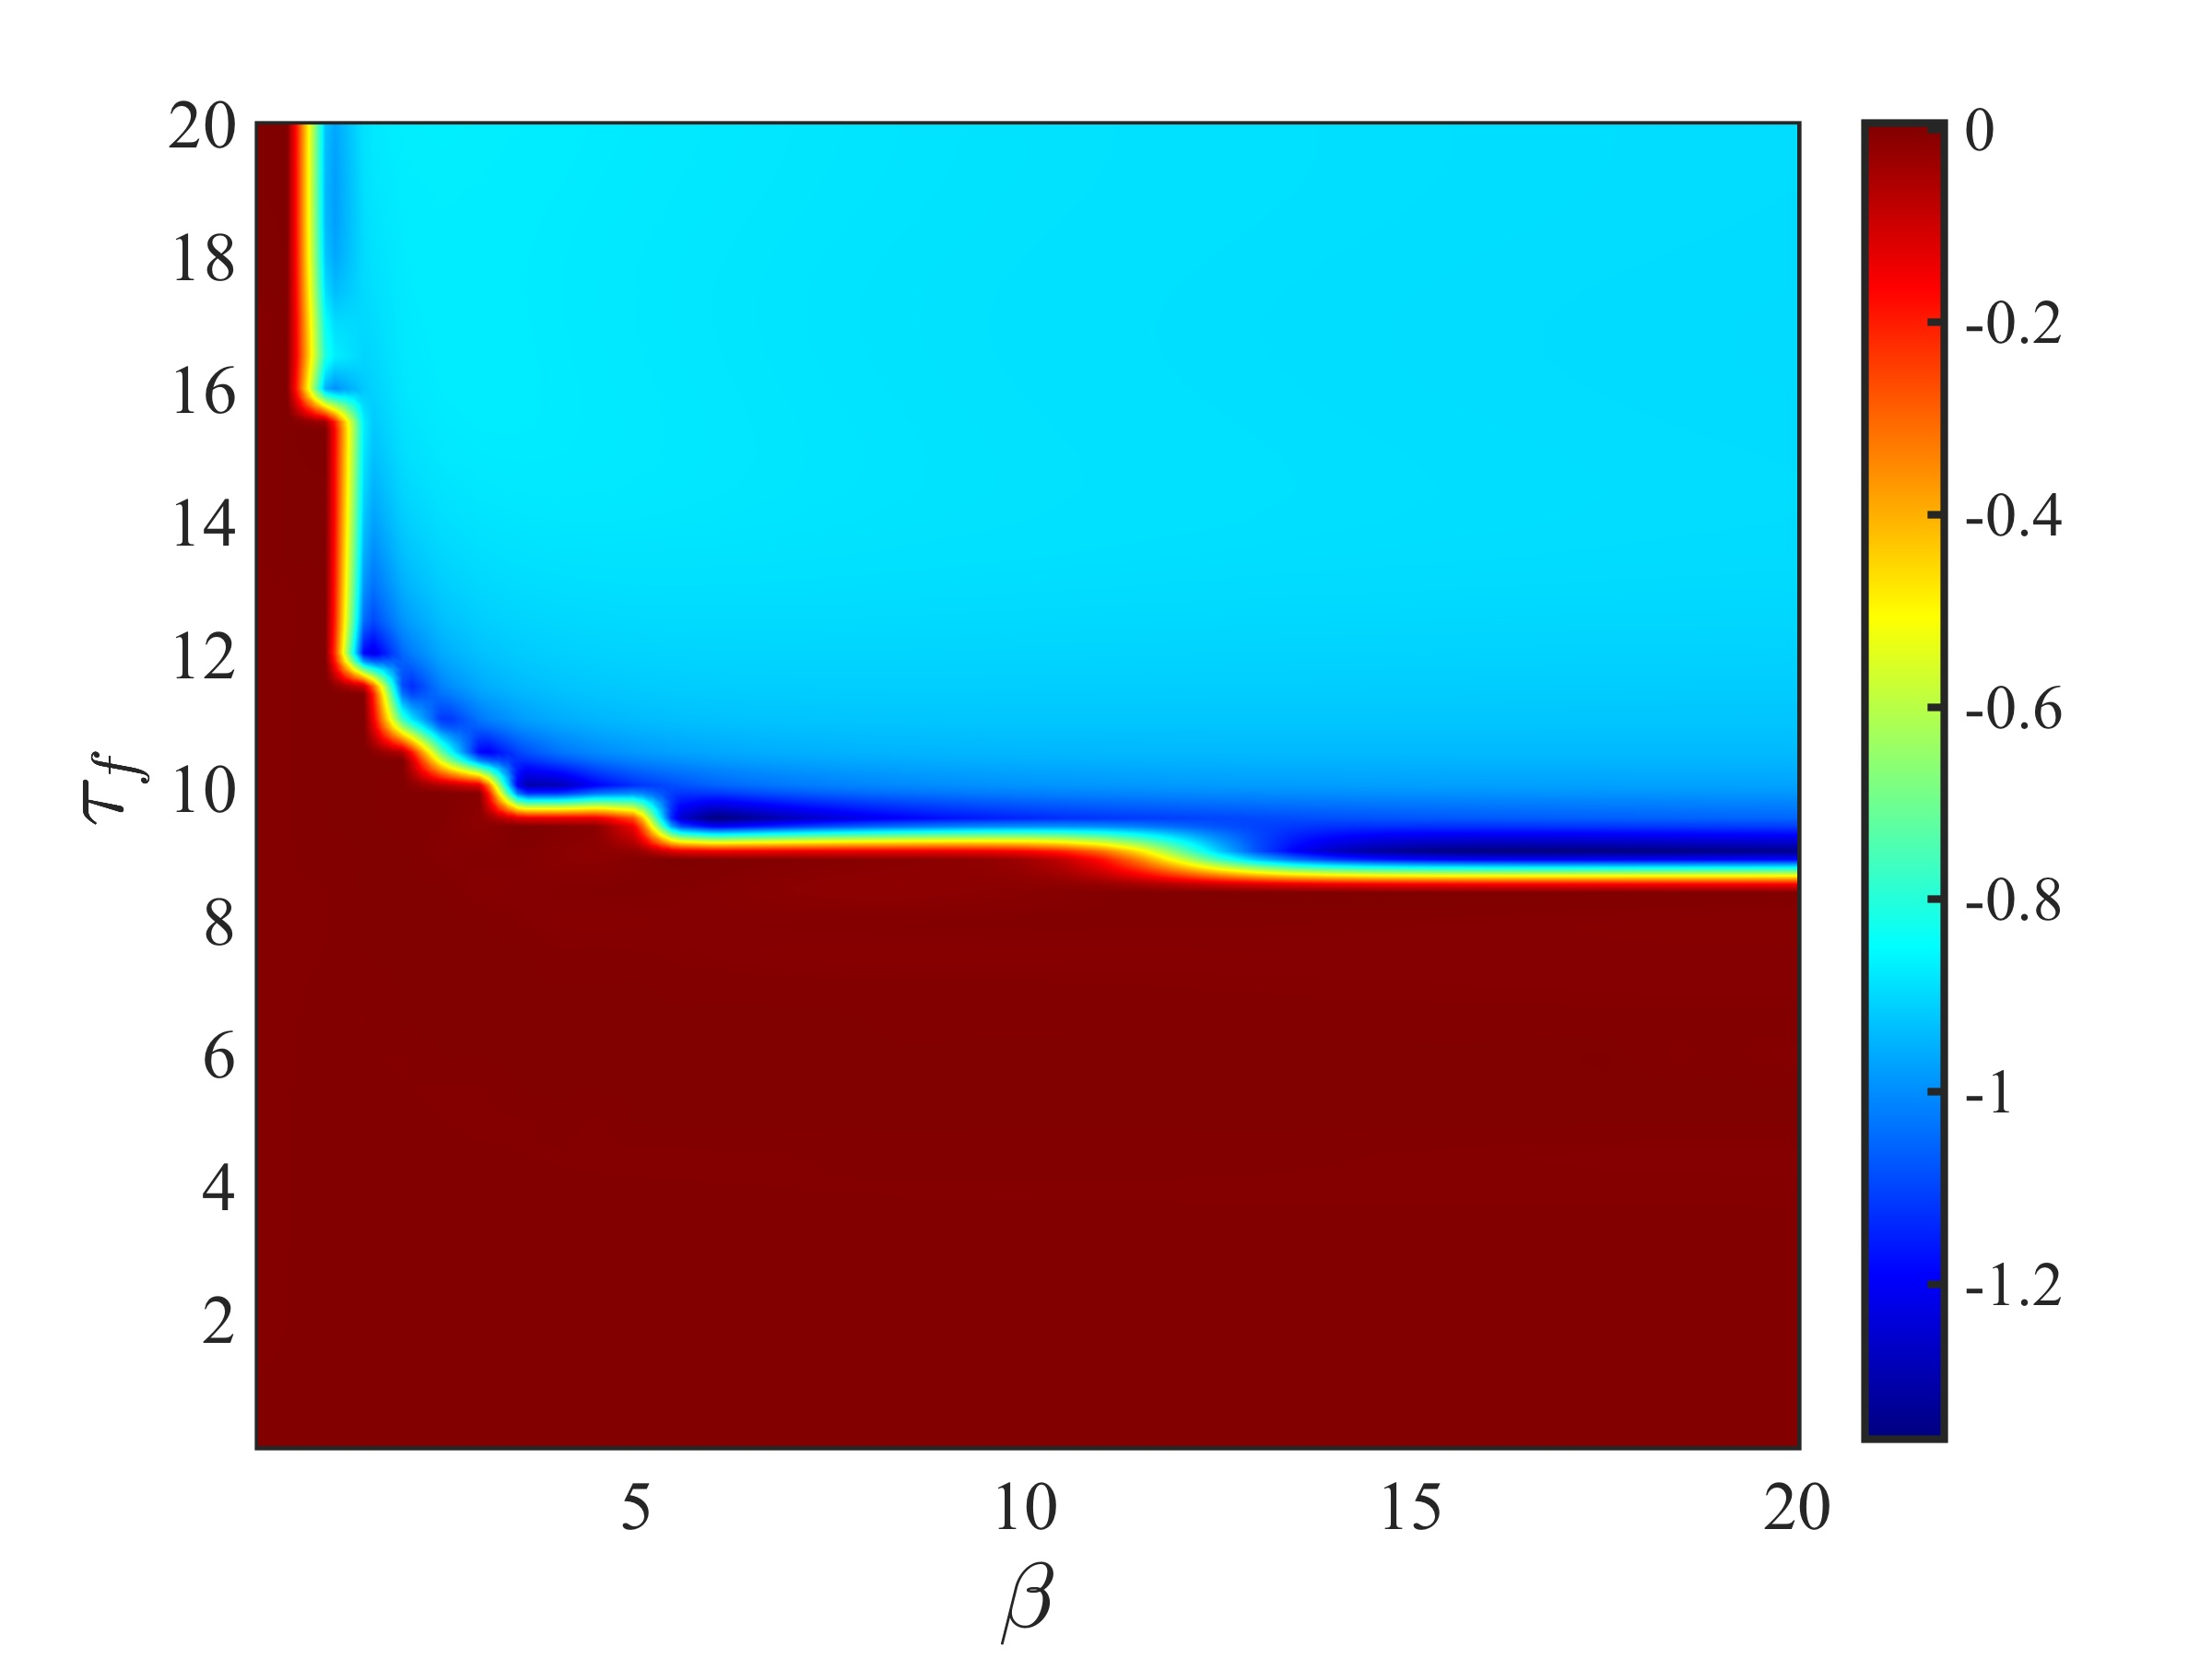
\includegraphics[width=4.2cm]{FatQOut.jpg} 
\\
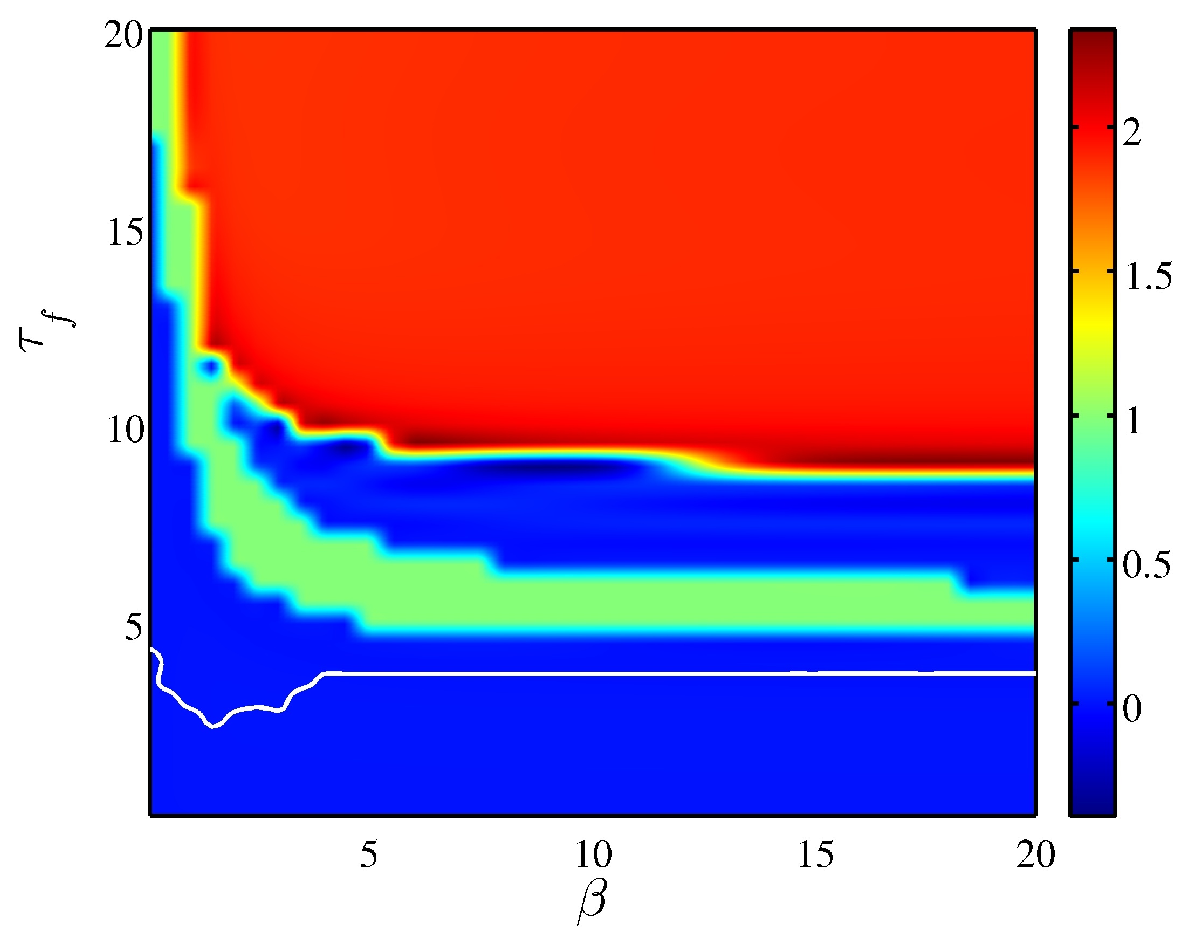
\includegraphics[width=8.5cm]{FatPDEvODE_rcg_t.eps} 
\vspace{-0.5em}
\caption[Power Ratios Inside and Outside Tweezer with Wide Width]{Power ratios as in Fig.~\ref{fig:SkinnyQ} but for a natural tweezer with width $\sigma_\phi = 2$ and height $h_\phi = 6.9949$.  The detuning for the system is $\Delta =  3.0859$.   Same layout as in Fig.~\ref{fig:SkinnyQ}.  The difference power ratio (c) defines the thresholds for a tweezed CS for all blue regions, a no-CS for all green regions, and non-tweezed for all orange regions.  
}
\label{fig:FatQ}
\end{figure}
%%%%%%%%%% Fig  %%%%%%%%%%%%%%%%%%%%%%%%%%%%%%%%%%%%%% 

As a sample of the dynamic properties of tweezability, Fig.~\ref{fig:Skinny1} depicts a sample for a tweezed CS while Fig.~\ref{fig:Skinny2} depicts a dissipative no-CS solution for the full LL model.  Figs.~\ref{fig:Skinny1}(a) and~\ref{fig:Skinny1}(b) depict the dynamic evolution of the LL model and NCVA, respectively, for the narrow tweezer $\tau_f = 0.1$ and $\beta=0.1$.   Figure~\ref{fig:Skinny1}(c) contains three snapshots of the system at $z=0$ (top panel), $z^*$ (middle panel), and 10 (bottom panel) for comparison between the LL model (solid (blue) line), the NCVA solution (solid (red) line) and the tweezer (solid (grey) line).  For an example of no-CS dynamic properties, Fig.~\ref{fig:Skinny2} for narrow tweezer $\tau_f = 2$ and $\beta=10$ is organized the same as Fig.~\ref{fig:Skinny1}.   In this example, the NCVA and the LL model admits a no-CS state.  It is also important to mention that the NCVA variational parameters for the narrow tweezer accurately capture the full LL model solution properties, such as height and width as seen in Figs~\ref{fig:Skinny1}(c) and ~\ref{fig:Skinny2}(c).




\subsection{Tweezer with Wide Width} 
\label{section:Fat}

In the last case study, we are interested in a tweezer with a wide width $\sigma_\phi = 3$ and height $h_\phi = 6.9949$ by Eq.~(\ref{height}).  For the full LL Eq.~(\ref{eq:LLETweeze}), the steady state CS is found centered at $\tau_0 = 0$ using a Newton-Krylov solver and the power-balance constraint Eq.~(\ref{LLConstraint}) which selects a particular detuning parameter $\Delta = 3.0859$ for the system.  The setup is the same as in the other examples.


%%%%%%%%%% Fig  %%%%%%%%%%%%%%%%%%%%%%%%%%%%%%%%%%%%%%
\begin{figure}[t!!]
\centering
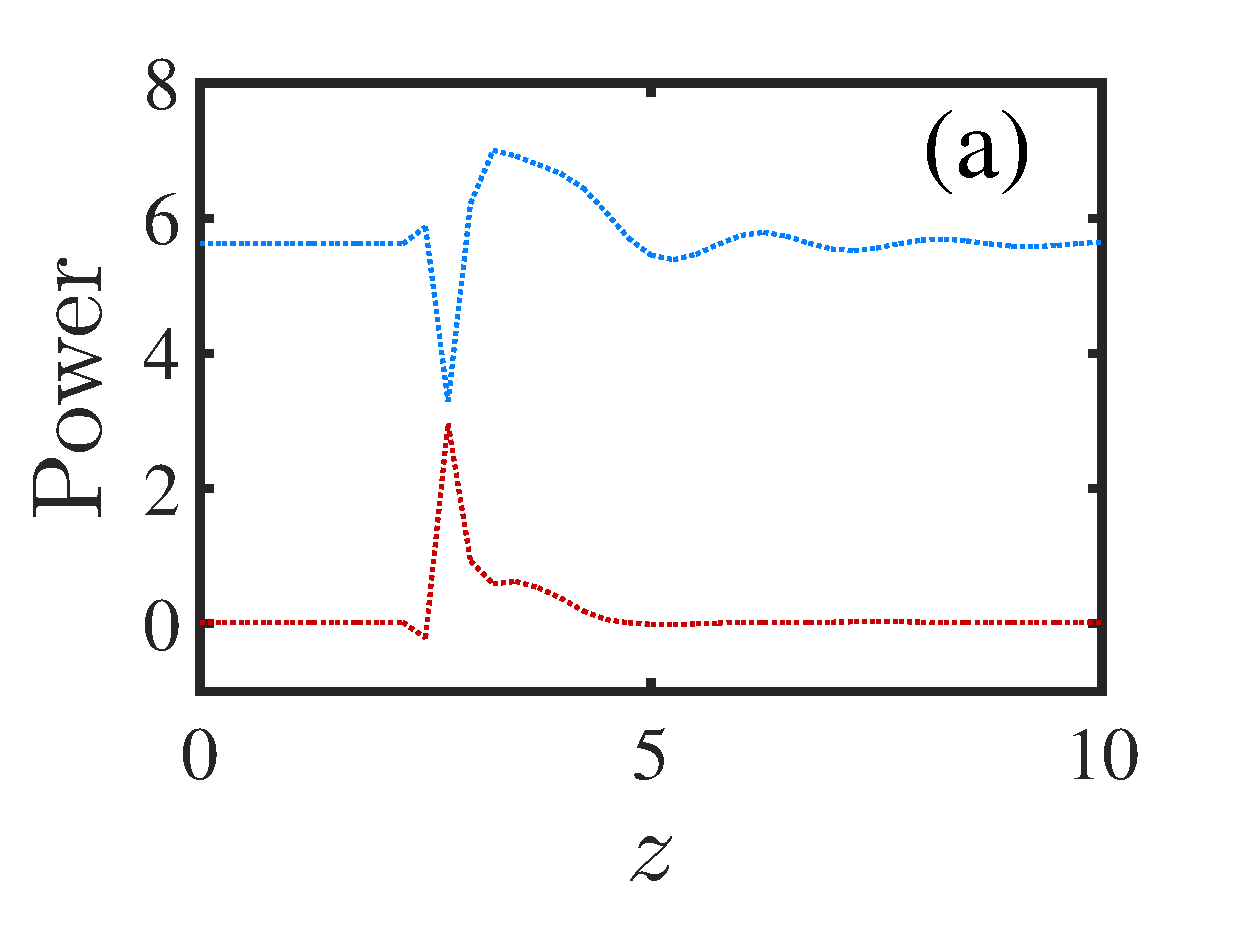
\includegraphics[width=4.2cm]{fatTimeMass1.eps} 
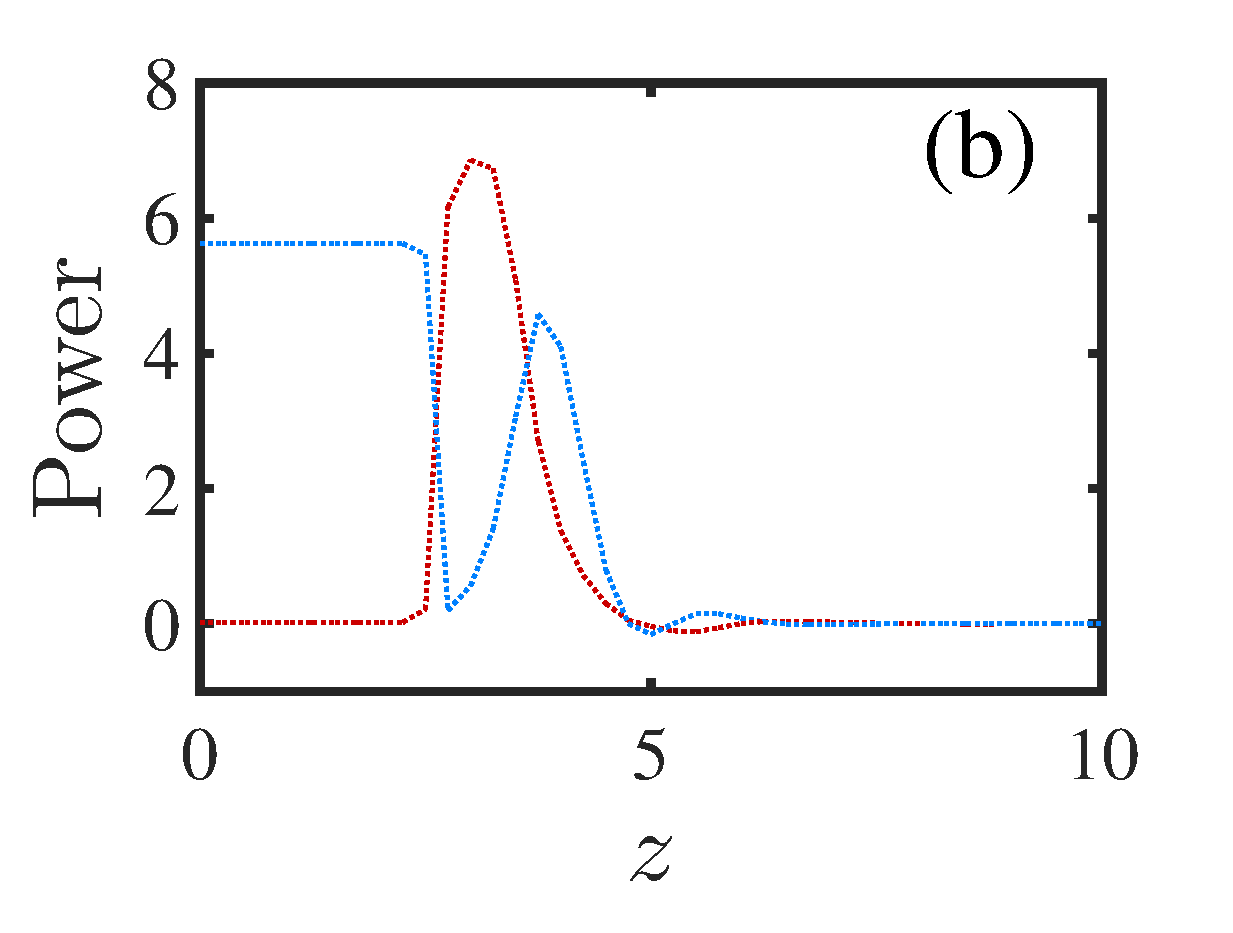
\includegraphics[width=4.2cm]{fatTimeMass2.eps} 
\\
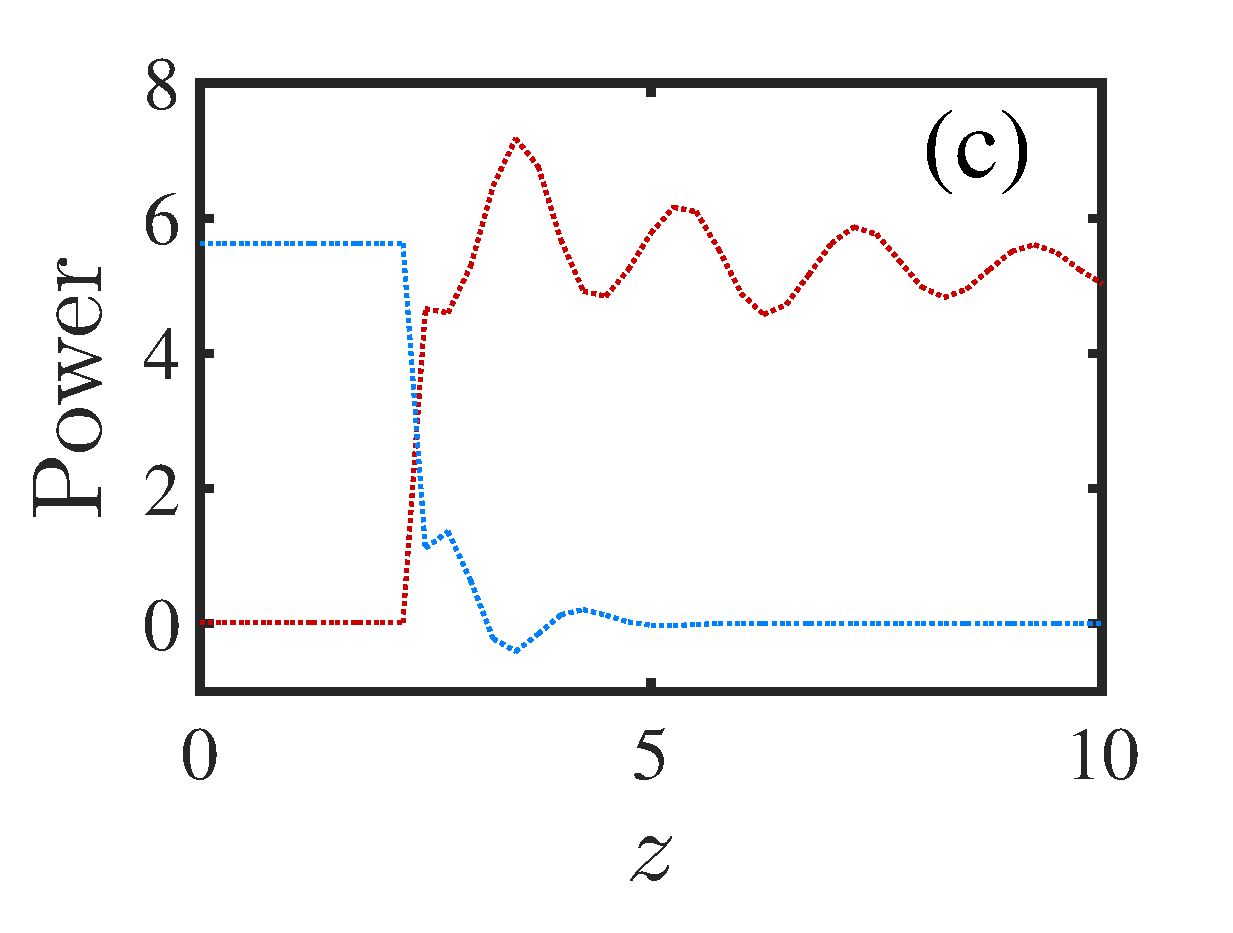
\includegraphics[width=4.2cm]{fatTimeMass3.eps} 
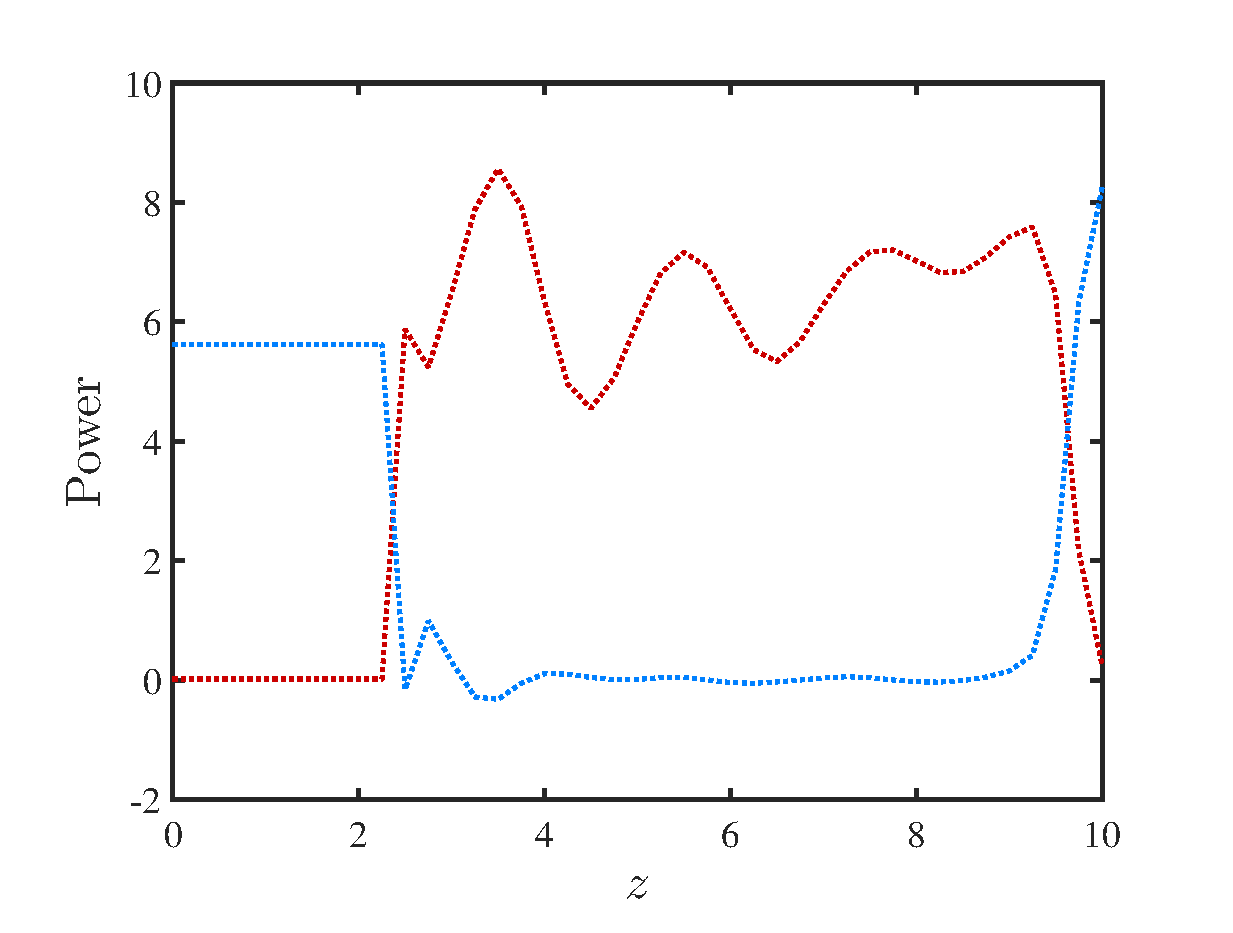
\includegraphics[width=4.2cm]{fatTimeMass5.eps}
\vspace{-0.5em}
\caption[Tweezer with Wide Width Power Comparison]{Comparison of the powers as in Fig.~\ref{fig:SkinnyComp} but for a wide tweezer.  Same layout as Fig.~\ref{fig:SkinnyComp}, but for parameters (a) $\tau_f = 4$ and $\beta=10$, (b) $\tau_f = 5.5$ and $\beta=10$, (c) $\tau_f = 18$ and $\beta=10$ and (d) $\tau_f = 9$ and $\beta=10$.  The left top panel (a) has no change in power inside or outside the tweezer which describes a tweezed CS, while right top panel (b) shows fluctuations caused by an uneven tweezing.  The left bottom panel (c) is an example of the tweezer moving too quickly and leaving the CS outside the tweezer.  The right bottom panel (d) is ``artificial'' tweezing, in which the trap initially loses the CS but but $z_f$ the CS catches up the tweezer.
}
\label{fig:FatComp}
\end{figure}
%%%%%%%%%% Fig  %%%%%%%%%%%%%%%%%%%%%%%%%%%%%%%%%%%%%%

%%%%%%%%%% Fig  %%%%%%%%%%%%%%%%%%%%%%%%%%%%%%%%%%%%%%
\begin{figure}[t!]
\centering
\hskip 0.4em 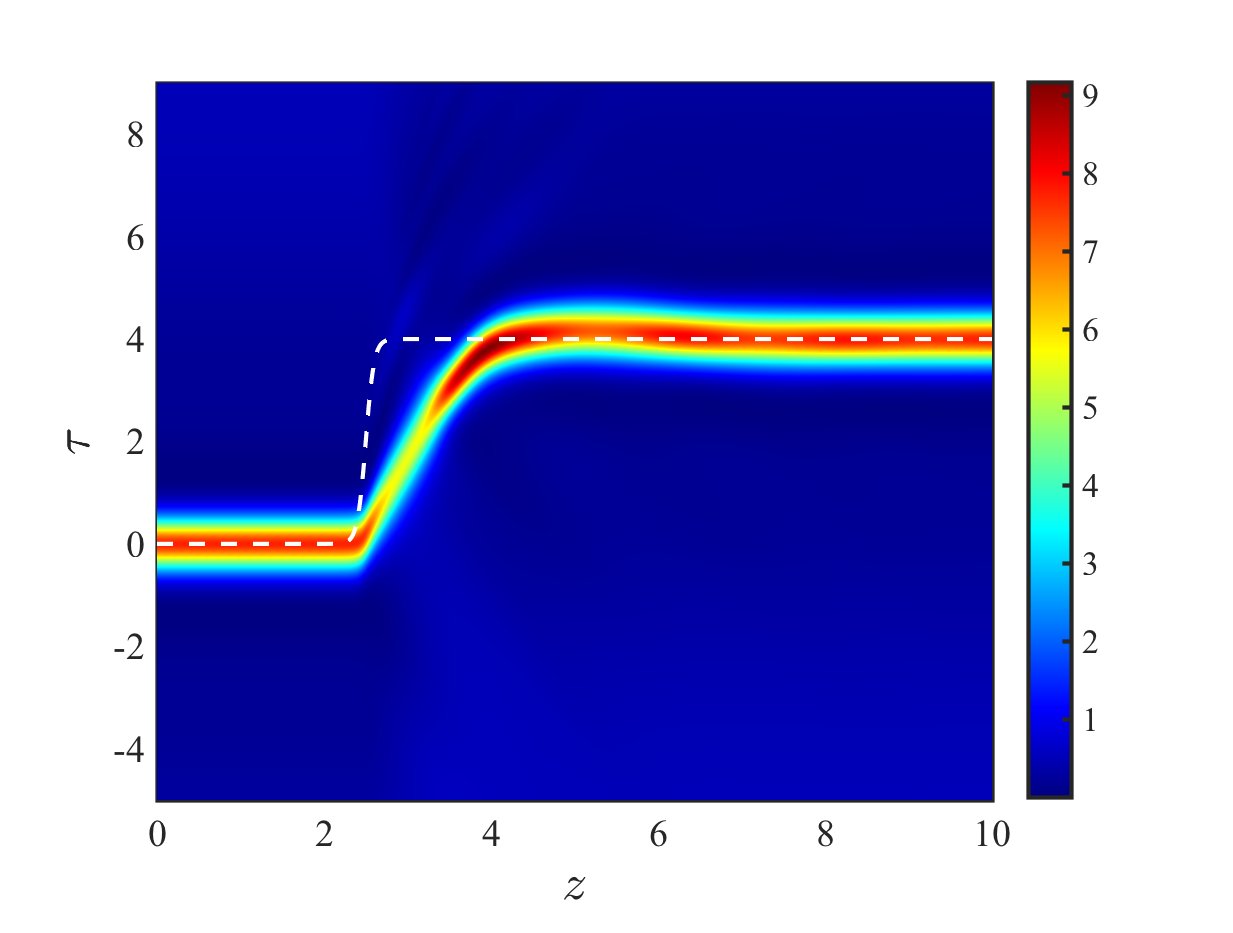
\includegraphics[width=4.2cm]{fatDensity1.eps} 
\hskip -0.5em 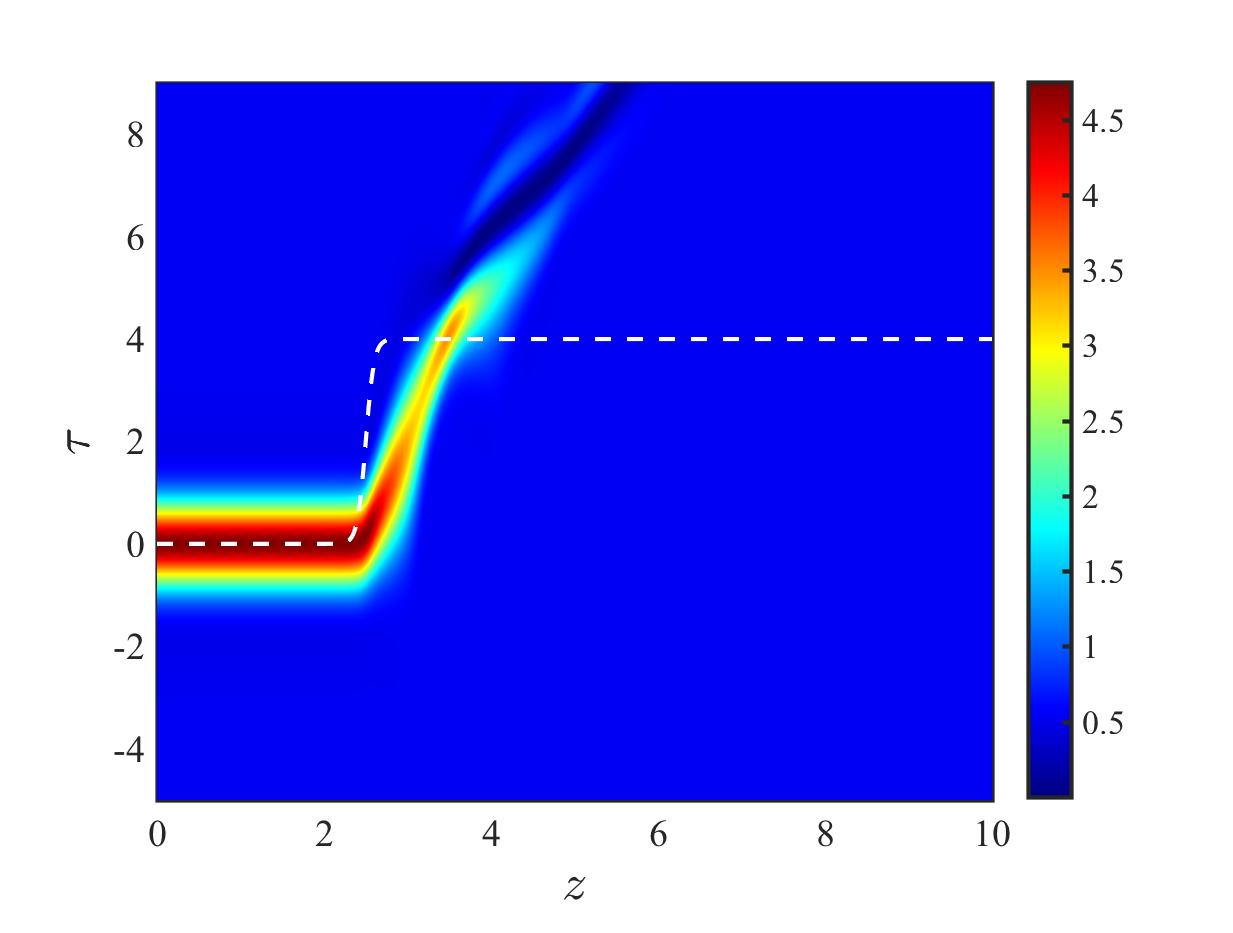
\includegraphics[width=4.2cm]{fatNCVADensity1.eps} 
\\
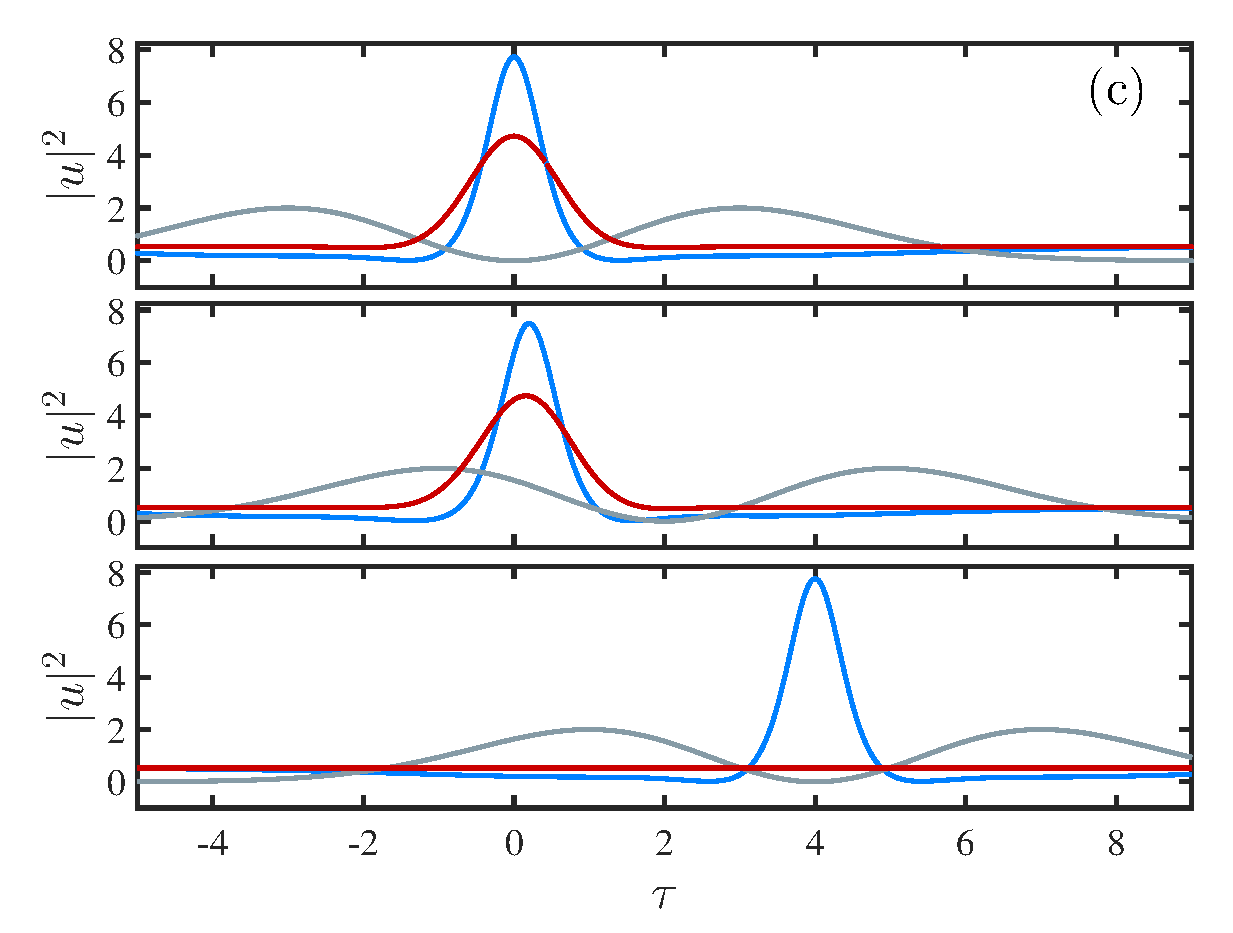
\includegraphics[width=8cm]{fatTimeSeries1.eps} 
\vspace{-0.5em}
\caption[Dynamic Evolution of Wide Tweezer with Tweezed CS]{Dynamic evolution as in Fig.~\ref{fig:Skinny1} but for $\tau_f = 4$ and $\beta = 10$.  Same layout as in Fig.~\ref{fig:Skinny1}.  In this sample, the NCVA solution is a no-CS, while the LL model is a tweezed-CS.
}
\label{fig:Fat1}
\end{figure}
%%%%%%%%%% Fig  %%%%%%%%%%%%%%%%%%%%%%%%%%%%%%%%%%%%%%


%%%%%%%%%% Fig  %%%%%%%%%%%%%%%%%%%%%%%%%%%%%%%%%%%%%%
\begin{figure}[b!]
\centering
\hskip 0.4em 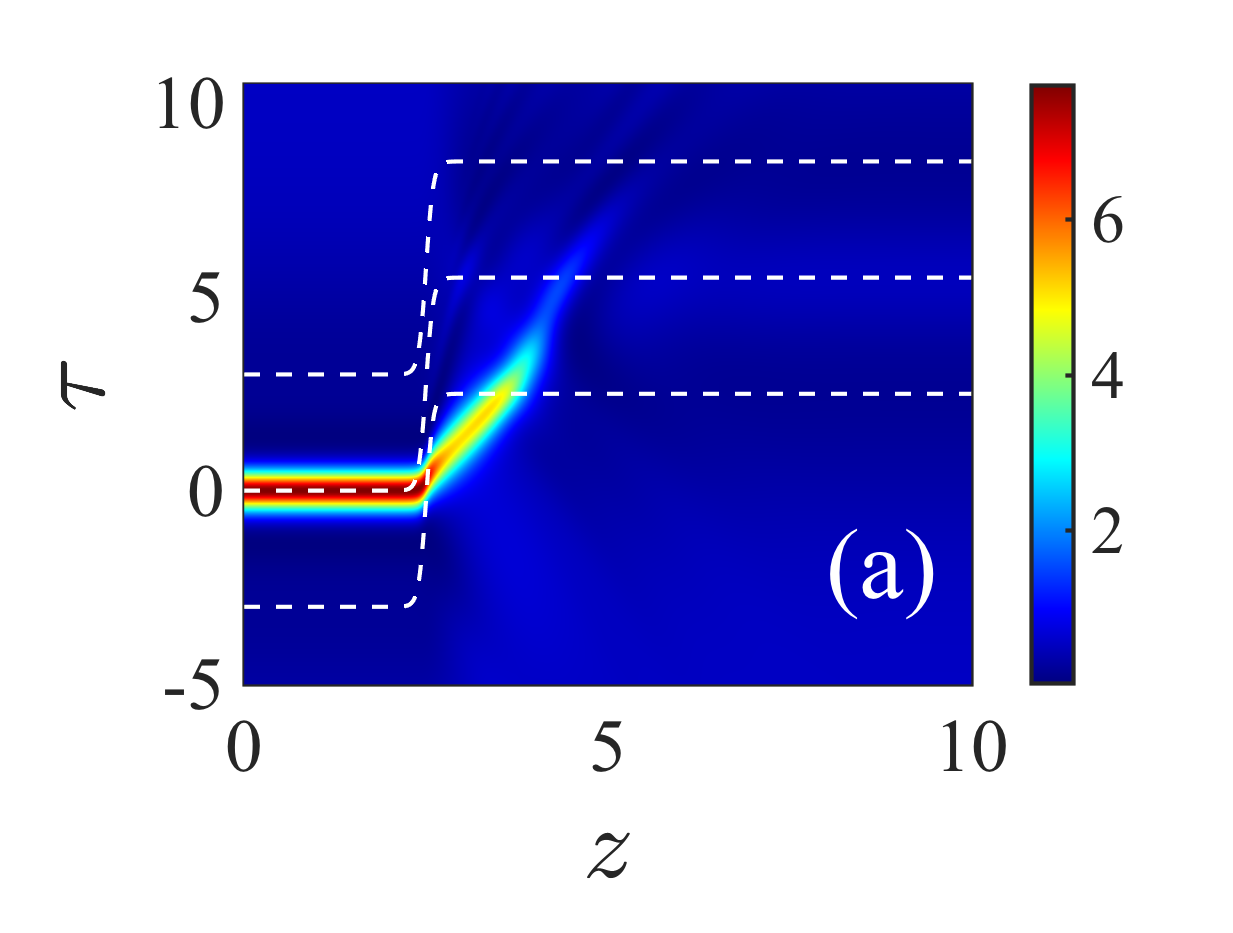
\includegraphics[width=4.2cm]{fatDensity2.eps} 
\hskip -0.5em 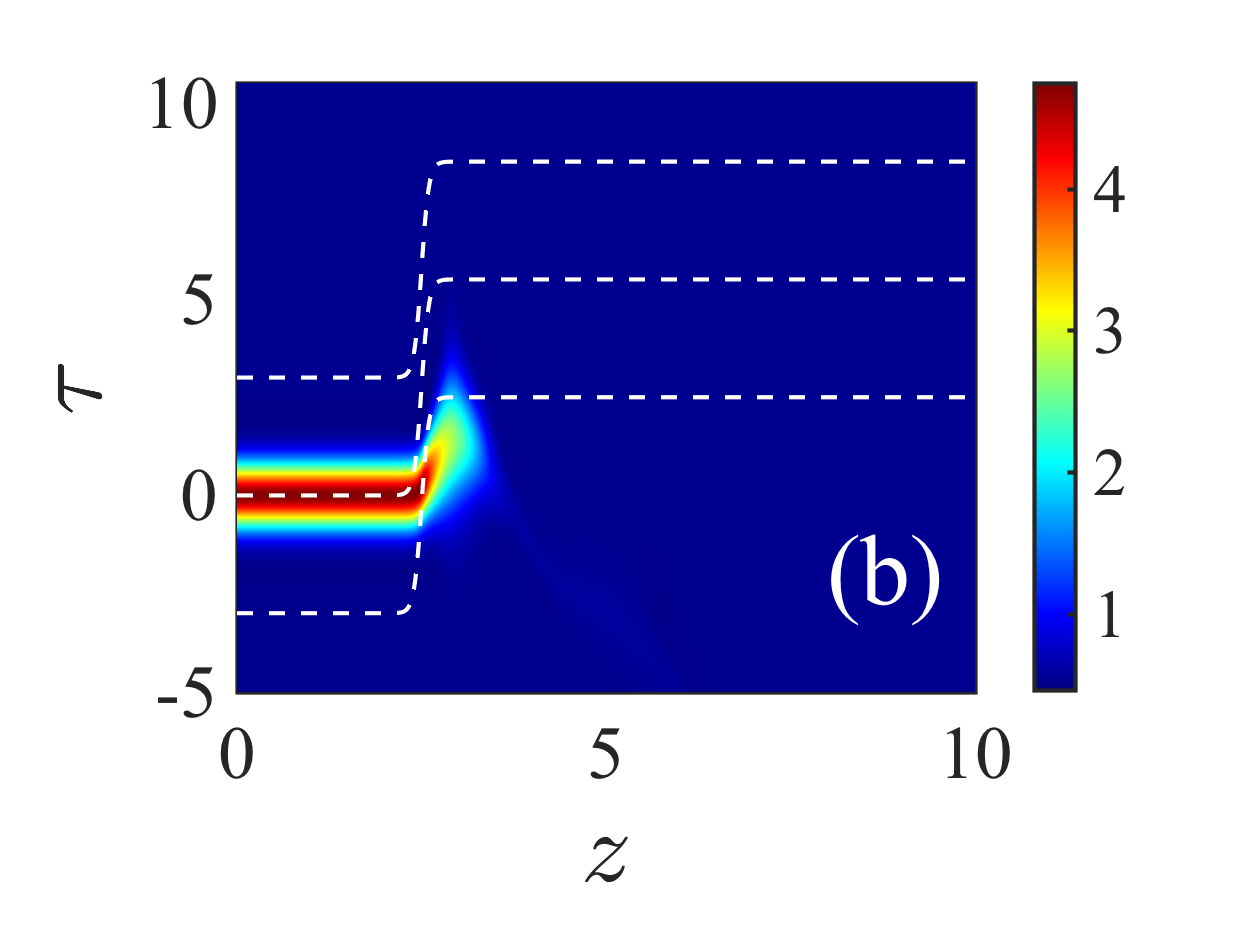
\includegraphics[width=4.2cm]{fatNCVADensity2.eps} %{fatNCVADensity2.eps} 
\\
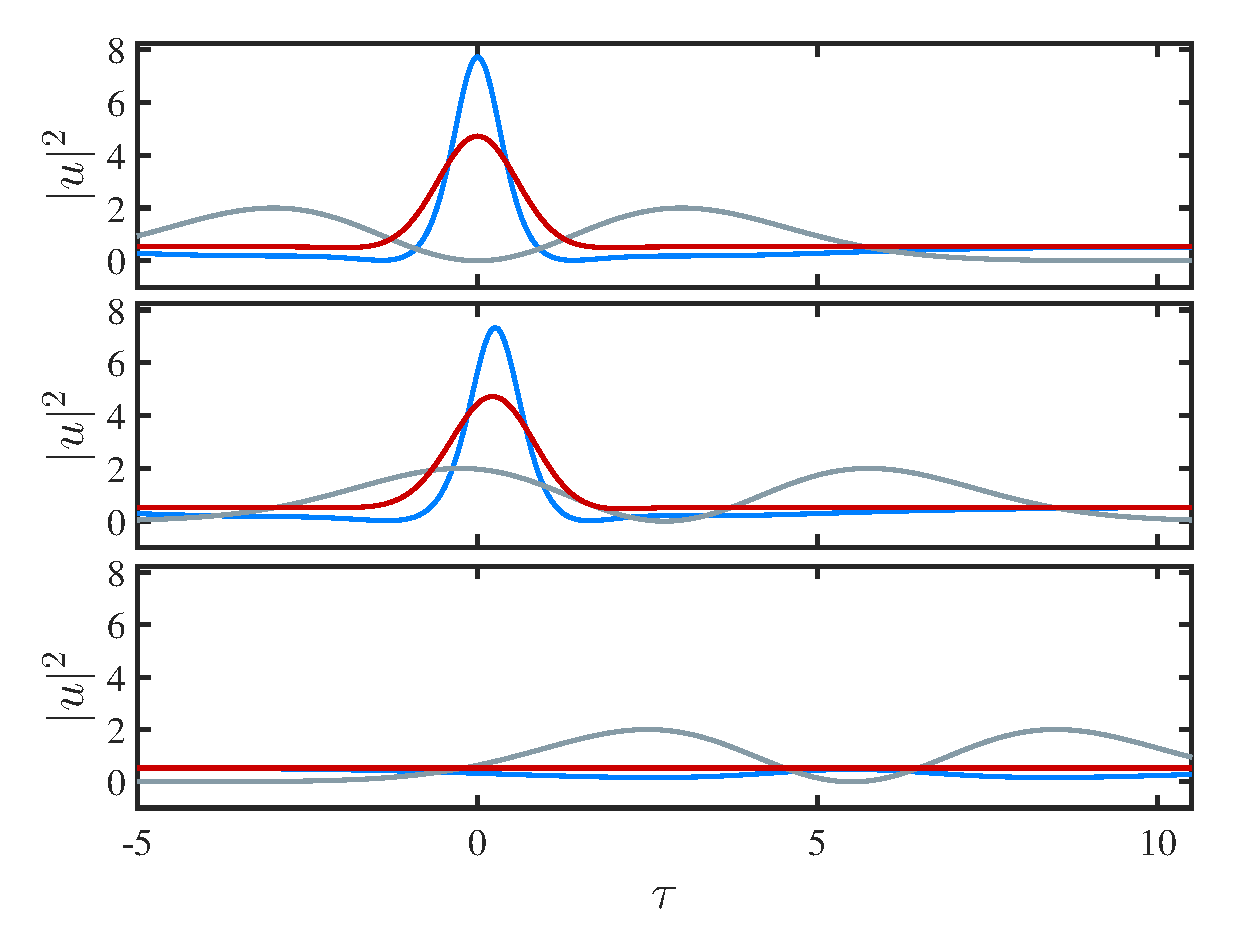
\includegraphics[width=8cm]{fatTimeSeries2.eps} 
\vspace{-0.5em}
\caption[Dynamic Evolution of Wide Tweezer with no-CS]{Dynamic evolution as in Fig.~\ref{fig:Skinny1} but for $\tau_f = 5.5$ and $\beta = 10$.  Same layout as in Fig.~\ref{fig:Skinny1}.  In this sample, the NCVA and the full LL model is a no-CS.  }
\label{fig:Fat2}
\end{figure}
%%%%%%%%%% Fig  %%%%%%%%%%%%%%%%%%%%%%%%%%%%%%%%%%%%%%

%%%%%%%%%% Fig  %%%%%%%%%%%%%%%%%%%%%%%%%%%%%%%%%%%%%%
%\begin{figure}[htb!]
%\centering
%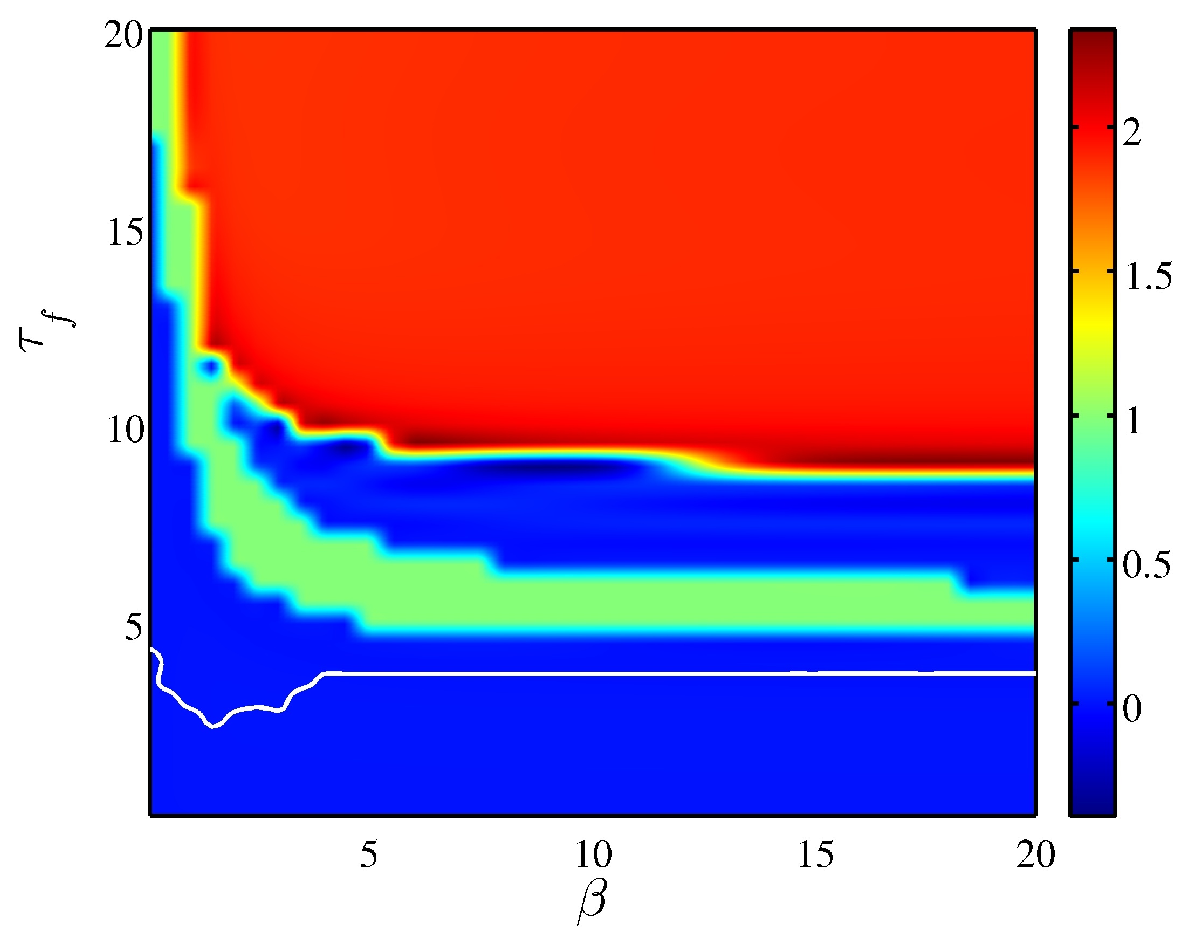
\includegraphics[width=8.5cm]{FatPDEvODE_rcg_t.eps}
%\caption[Comparison of Power Ratio Inside Wide Tweezer for LL Model and NCVA]{Comparison of difference in power ratios between the NCVA and LL model as in Fig.~\ref{fig:SkinnyVsNCVA} but for a wide tweezer.  Same layout as Fig.~\ref{fig:SkinnyVsNCVA}.  The NCVA distinguishes a threshold between tweezed and no-CS solution at $\tau_f\approx 4$.  The LL model displays tweezed CSs in the blue region (under the green region), no-CSs in the green region, and a non-tweezed CSs in red region.  The blue region between the green and red regions is ``artificial'' tweezing, in which the trap initially loses the CS but at $z_f$ the CS catches up and is re-trapped by the tweezer.
%}
%\label{fig:fatVsNCVA}
%\end{figure}
%%%%%%%%%% Fig  %%%%%%%%%%%%%%%%%%%%%%%%%%%%%%%%%%%%%%


Figure~\ref{fig:FatQ} depicts the density of the power ratios as well as the difference Fig.~\ref{fig:FatQ} with the same layout as Fig.~\ref{fig:SkinnyQ} but for the wide tweezer.  The wide tweezer is defined by three fundamental evolutions: a tweezed CS for all $\beta$ when $0<\tau_f < 5$, no-CS for most $\beta$ when $5<\tau_f <14$, and a non-tweezed CS for all $\beta$ when $\tau_f > 14$.  The threshold for the existence of the tweezed CS with a wide tweezer is only marginally larger than that found for a natural width tweezer.  Using the same layout as Fig.~\ref{fig:SkinnyQ}, Fig.~\ref{fig:FatQ} compares the difference in quotient ratios between the NCVA and the full LL model.  The NCVA threshold between the tweezed CS and no-CS is approximately by $\tau_f = 4$ while the LL model has a threshold around $\tau_f = 5$ for most values of $\beta$.  

In order to better explain the power ratio, we examine four examples of the power inside $P_{\rm I}$ Eq.~(\ref{Pin}) and outside $P_{\rm O}$ Eq.~(\ref{Pout}) for $\beta = 10$ with $\tau_f = 4$, 5.5, 9, and 18 in Fig.~\ref{fig:FatComp}.  In Fig.~\ref{fig:FatComp} the red lines are $P_{\rm I}$ and the blue lines are $P_{\rm O}$.  Panel (a), $\beta = 10$ at $\tau_f = 4$, depicts a case that has no change in power inside or outside the tweezer which describes a tweezed CS, while panel (b), $\beta = 5.5$ at $\tau_f = 10$, shows complete loss of power inside which describes a no-CS.  Panel (c), $\beta = 10$ at $\tau_f = 18$, depicts an example of the non-tweezed CS.  Panel (d), for $\beta = 10$ and $\tau_f = 9$, depicts an ``artificially'' tweezed CS defined by the complete loss of the CS from the trap, but rather than a stationary CS left outside the trap (as is the case in non-tweezed CS), the CS is imparted with enough energy to continue moving in the direction of the tweezer.  By the final time $z_f$, the CS catches up and it is re-trapped by the tweezer and results in $P_{\rm I} \approx 1$ despite this case not being a true tweezed CS. 


%%%%%%%%%% Fig  %%%%%%%%%%%%%%%%%%%%%%%%%%%%%%%%%%%%%%
\begin{figure}[t!]
\centering
\hskip 0.4em 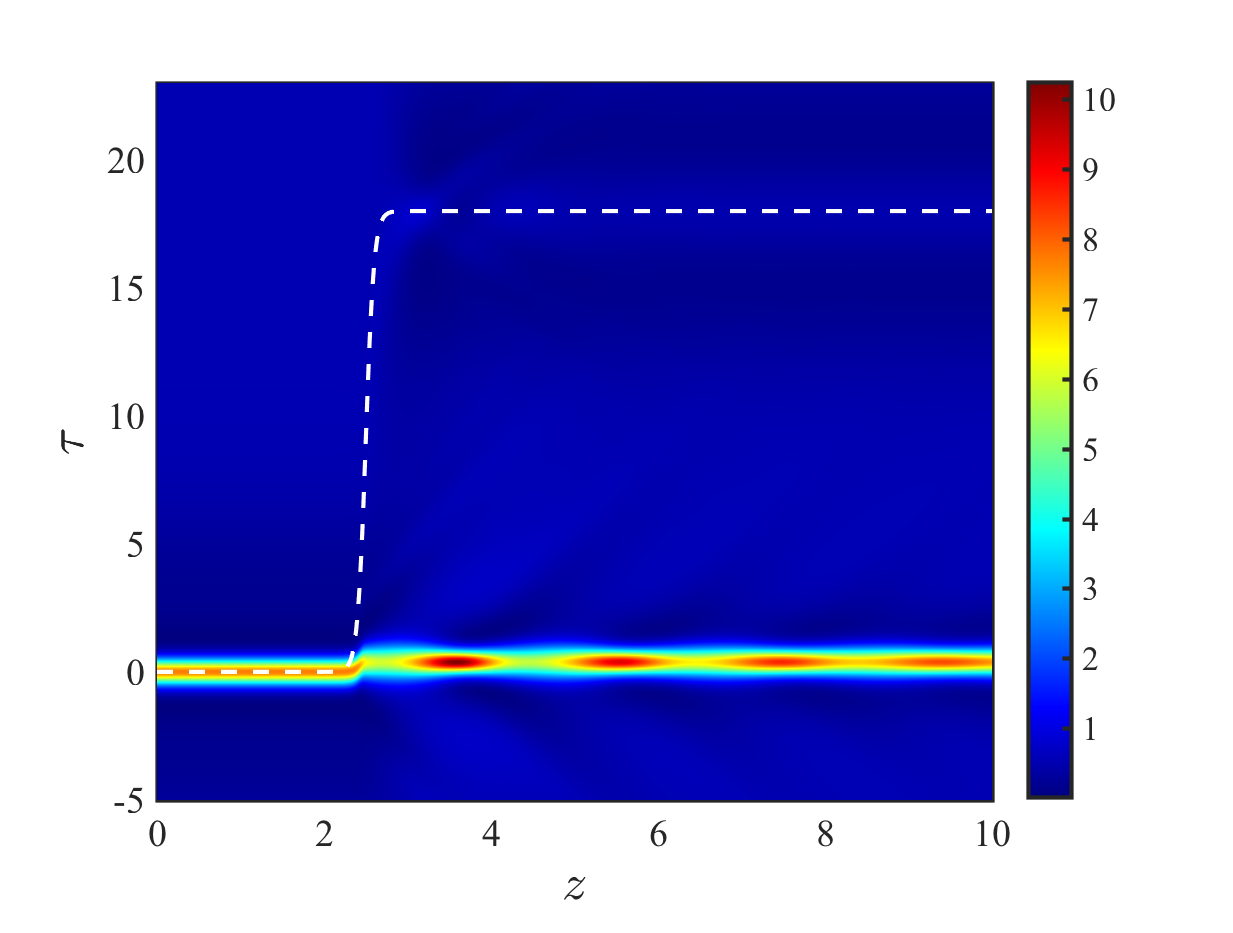
\includegraphics[width=4.2cm]{fatDensity3.eps} 
\hskip -0.5em 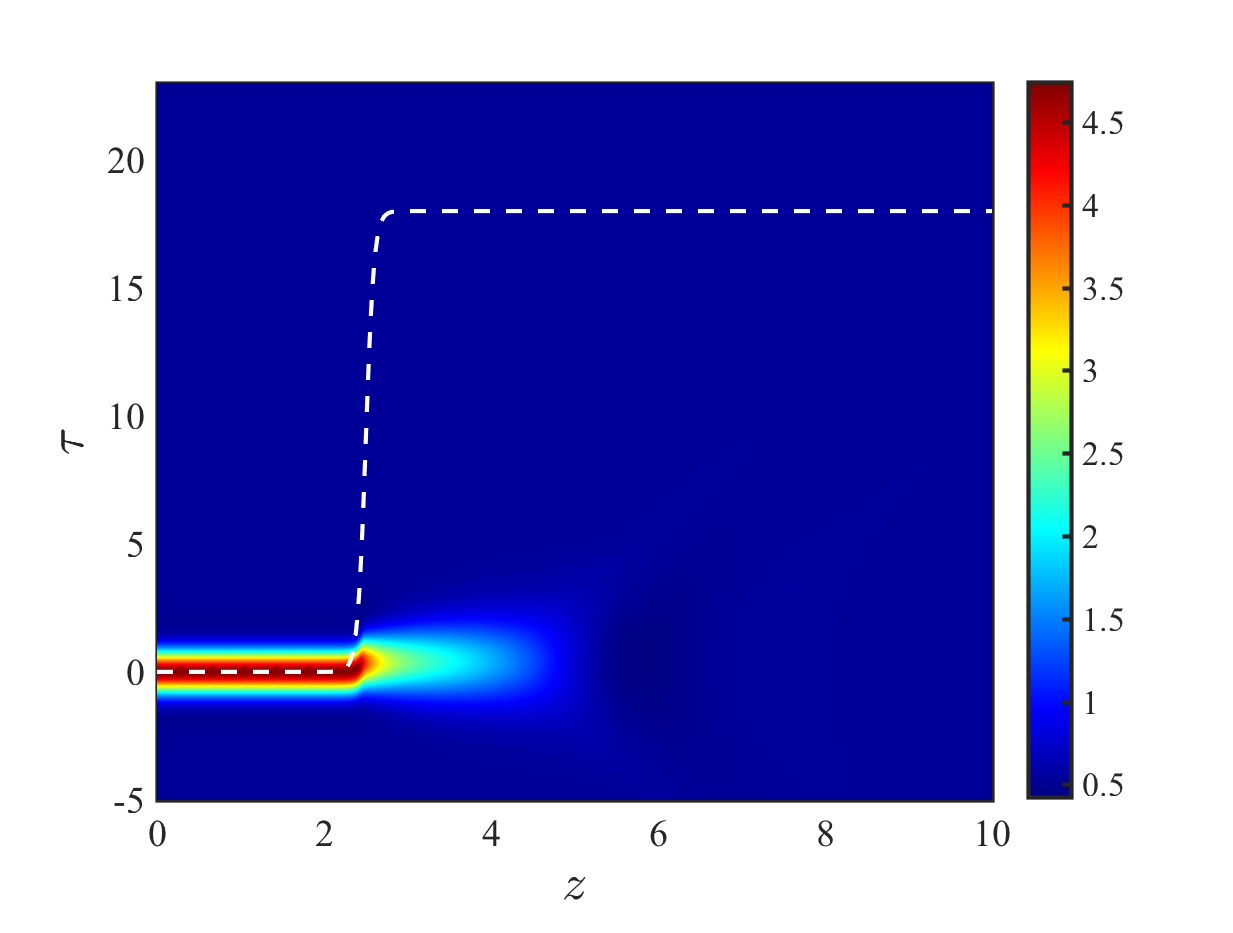
\includegraphics[width=4.2cm]{fatNCVADensity3.eps} %{fatNCVADensity3.eps} 
\\
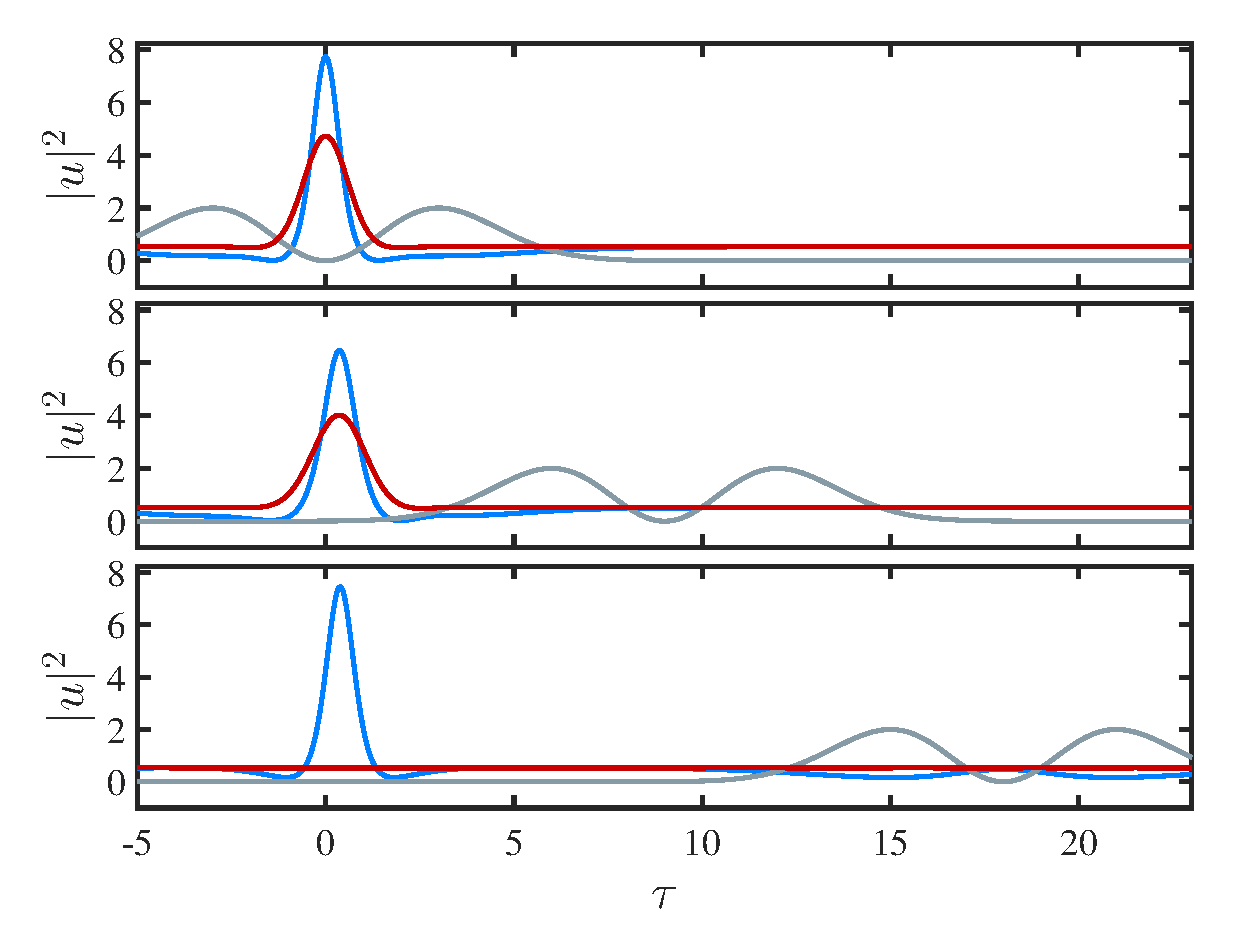
\includegraphics[width=8cm]{fatTimeSeries3.eps} 
\vspace{-0.5em}
\caption[Dynamic Evolution of Wide Tweezer with Non-Tweezed CS]{Dynamic evolution as in Fig.~\ref{fig:Skinny1} but for $\tau_f = 18$ and $\beta = 10$.  Same layout as in Fig.~\ref{fig:Skinny1}.  In this sample, the NCVA solution is a no-CS.  The non-tweezed CS of the LL model is stationary outside the wide tweezer, which leaves the CS behind as the phase modulation is moved.
}
\label{fig:Fat3}
\end{figure}
%%%%%%%%%% Fig  %%%%%%%%%%%%%%%%%%%%%%%%%%%%%%%%%%%%%%

%%%%%%%%%% Fig  %%%%%%%%%%%%%%%%%%%%%%%%%%%%%%%%%%%%%%
\begin{figure}[t!]
\centering
\hskip 0.4em 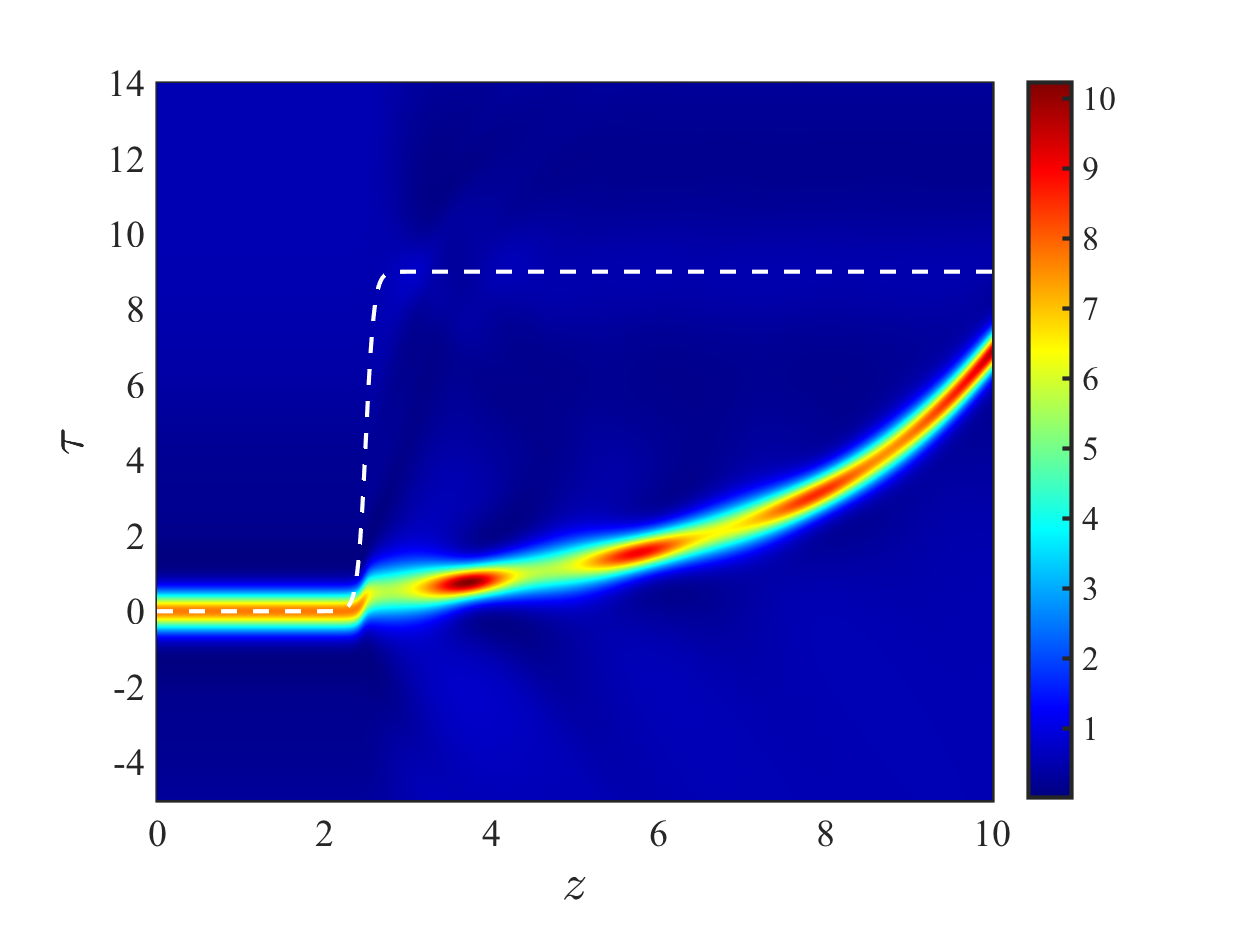
\includegraphics[width=4.2cm]{fatDensity5.eps} 
\hskip -0.5em 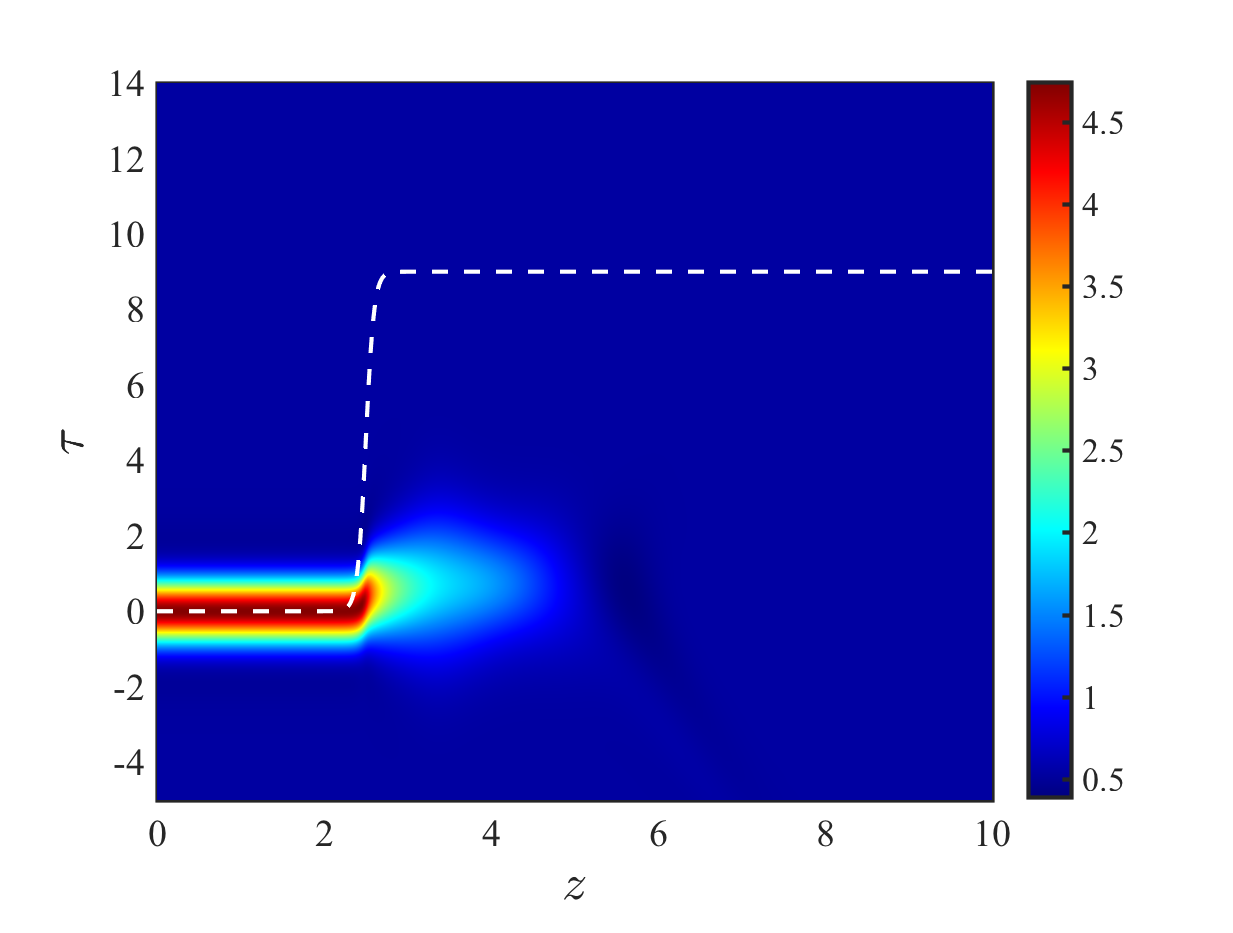
\includegraphics[width=4.2cm]{fatNCVADensity5.eps} 
\\
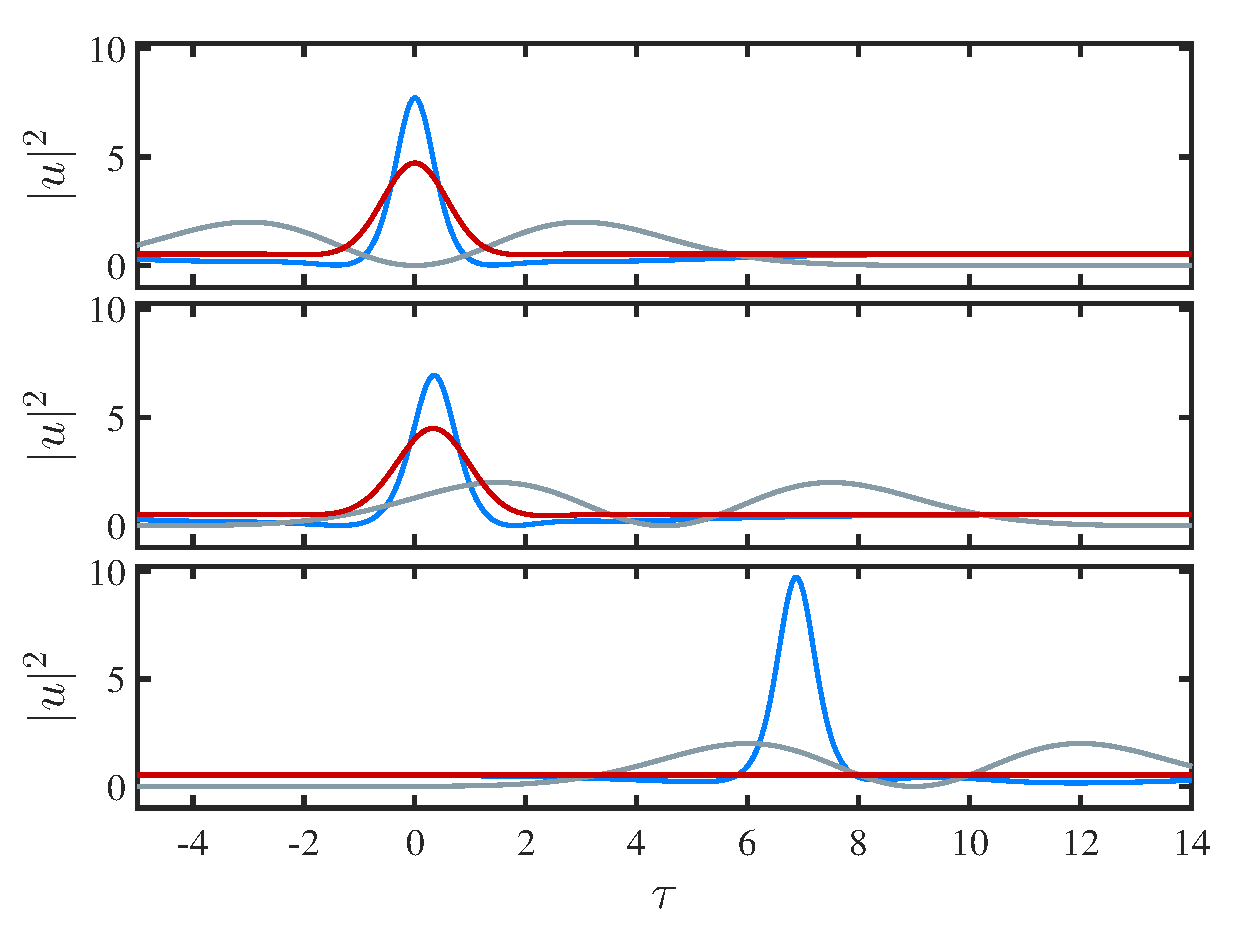
\includegraphics[width=8cm]{fatTimeSeries5.eps} 
\vspace{-0.5em}
\caption[Dynamic Evolution of Wide Tweezer with Artificial Tweezing]{Dynamic evolution as in Fig.~\ref{fig:Skinny1} but for $\tau_f = 9$ and $\beta = 10$.  Same layout as in Fig.~\ref{fig:Skinny1}.  In this example, the NCVA is a no-CS.  The LL model has an ``artificially'' tweezed CS defined by the complete loss of the CS from the trap, but rather than a stationary CS left outside the trap (as is the case in non-tweezed CS), the CS is imparted with enough energy to continue moving in the direction of the tweezer.  By the final time $z_f$ the CS catches up with the tweezer and LL solutions are both no-CS. 
}
\label{fig:Fat4}
\end{figure}
%%%%%%%%%% Fig  %%%%%%%%%%%%%%%%%%%%%%%%%%%%%%%%%%%%%%


As a sample of the dynamic properties of tweezability, Fig.~\ref{fig:Fat1} depicts a tweezed CS in the LL model and no-CS in the NCVA.  Figure~\ref{fig:Fat2} shows a no-CS for both the full LL model and the NCVA.  For the third sample, Fig.~\ref{fig:Fat3} the tweezer leaves the CS outside the effective potential in the full LL model while in the NCVA the solution is dissipative.  In contrast, Fig.~\ref{fig:Fat4} depicts the existence of artificial tweezing in the full LL model and a no-CS in the NCVA.  As Figs.~\ref{fig:Fat1}(a) and (b) show the initial state [see solid (blue) line LL model solution and solid (red) line NCVA solution in Fig.~\ref{fig:Fat1}(c) top panel] is manipulated by the wide tweezer towards $\tau_f$ at speed $\beta$ [see solid (blue) line LL model solution  and solid (red) line NCVA solution in Fig.~\ref{fig:Fat1}(c) bottom panel], which we refer to as a tweezed CS in the LL model and a no-CS in the NCVA.  Figures~\ref{fig:Fat2}(a) and (b) show the initial state [see solid (blue) line LL model solution and solid (red) line NCVA solution in Fig.~\ref{fig:Fat2}(c) top panel] is dragged by the wide tweezer for a short time before being lost in the LL model whereas the NCVA is only a no-CS solution [see solid (blue) line LL model solution and solid (red) line NCVA solution in Fig.~\ref{fig:Fat2}(c) bottom panel].  As Figs.~\ref{fig:Fat3}(a) and (b) show the initial state [see solid (blue) line LL model solution and solid (red) line NCVA solution in Fig.~\ref{fig:Fat3}(c) top panel] is left behind as the wide tweezer is displaced for the LL model and is completely lost in the case of the NCVA  [see solid (blue) line LL model solution  and solid (red) line NCVA solution in Fig.~\ref{fig:Fat3}(c) bottom panel].  For the artificial tweezing dynamic properties, Figs.~\ref{fig:Fat4}(a) and (b) show the initial state [see solid (blue) line LL model solution and solid (red) line NCVA solution in Fig.~\ref{fig:Fat4}(c) top panel] is manipulated by the wide tweezer towards $\tau_f$ at speed $\beta$ [see solid (blue) line LL model solution and solid (red) line NCVA solution in Fig.~\ref{fig:Fat4}(c) bottom panel], and as the CS is dragged the solution is initial lost in the LL model, but catches back up and is re-trapped by the tweezer at $z_f$. 

